\chapter{MIPS Processors}
%%%%%%%%%%%%%%%%%%%%%%%%%%%%%%%%%%%%%%%%%%%%%%%%%%%%%%%%%%%%%%%%%%%%%%%%%%%%%%%%
%%%%%%%%%%%%%%%%%%%%%%%%%%%%%%%%%%%%%%%%%%%%%%%%%%%%%%%%%%%%%%%%%%%%%%%%%%%%%%%%
%%%%%%%%%%%%%%%%%%%%%%%%%%%%%%%%%%%%%%%%%%%%%%%%%%%%%%%%%%%%%%%%%%%%%%%%%%%%%%%%
\section {MIPS architecture}
The MIPS (microprocessor without interlocked pipeline stages) architecture is
based on an ISA, meaning that a very strict link between ISA (software) and
processor architecture (hardware) takes place.
%%%%%%%%%%%%%%%%%%%%%%%%%%%%%%%%%%%%%%%%%%%%%%%%%%%%%%%%%%%%%%%%%%%%%%%%%%%%%%%%
%%%%%%%%%%%%%%%%%%%%%%%%%%%%%%%%%%%%%%%%%%%%%%%%%%%%%%%%%%%%%%%%%%%%%%%%%%%%%%%%
%%%%%%%%%%%%%%%%%%%%%%%%%%%%%%%%%%%%%%%%%%%%%%%%%%%%%%%%%%%%%%%%%%%%%%%%%%%%%%%%
\subsection{Instruction set architecture}
For simple processor the instruction set is very basic, all instructions can be
classified in:
\begin{itemize}
  \item \textbf{R-type}: input and output are registers. Assembler syntax is
    something like: \verb|sub $1 $2 $3|.\\
    \textit{Format:}
    \begin{verbatim}
    |opcode(6 bit)|r_s(5 bit)|r_t(5 bit)|r_d (5 bit)|- (5 bit)|fz(6 bits)|
    \end{verbatim}
    Every single instruction always takes 32 bits (fixed format), these bit can
    be divided into 6 parts:
    \begin{itemize}
    \item $r_s, r_t$: source register.
    \item $r_d$: destination register.
    \item $fz$: opcode extension.
    \end{itemize}
    Since all registers are pointed using 5 bit, in a MIPS architecture like
    this there may be at maximum 32 registers.
  \item \textbf{Mem-type}: load and store data from memory, all other operations
    are performed starting from registers.
    An example is \verb|lw  $2, 20($1)| that corresponds to a word load where
    \$2 is the destination register and the source (i.e. the memory address
    referring to the location to be loaded) is given by: 20(\$1), which stands
    for taking the value in register \$1 (base address) and add a fixed
    offset (20).
    \begin{center}
      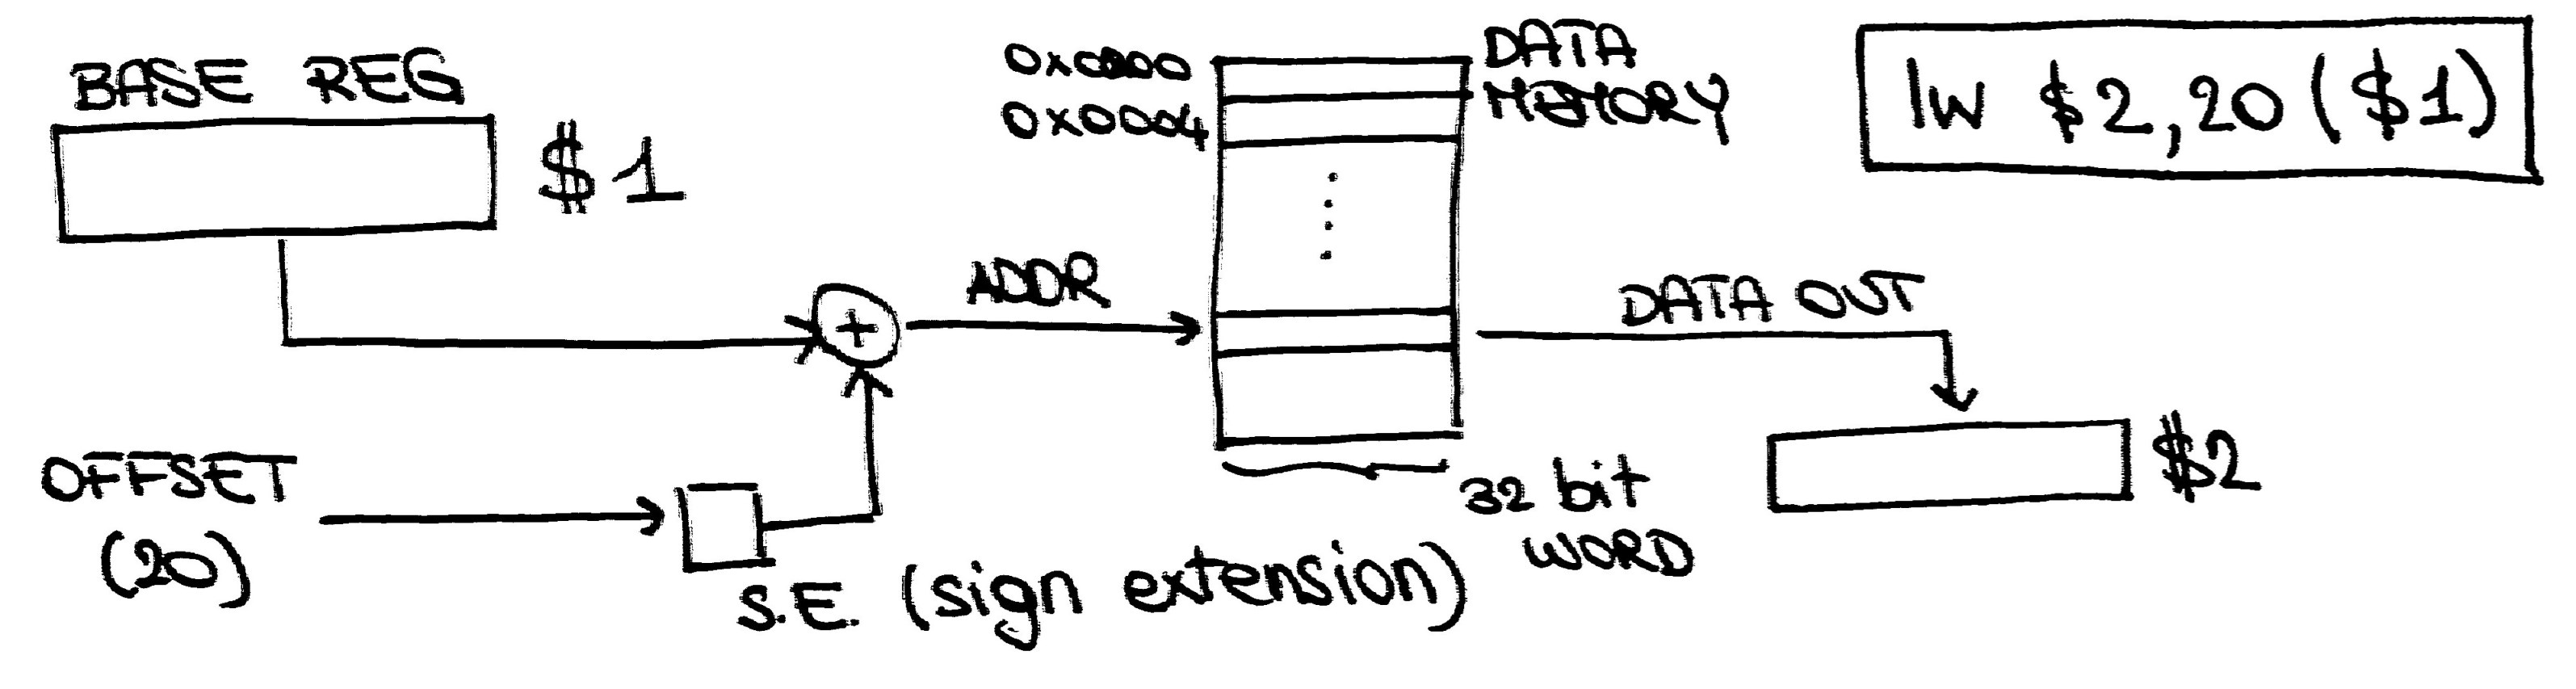
\includegraphics[width=0.8\linewidth]{img/img3/1}
    \end{center}
    \textit{Format:}
    \begin{verbatim}
    |opcode (6 bit)|R_s(5 bit)|r_t(5 bit)|offset (16 bit)|
    \end{verbatim}
    Where:
    \begin{itemize}
      \item $r_s$: base register (\$1).
      \item $r_t$: destination register (\$2).
      \item $offset$ (20).
    \end{itemize}
    Since the data expected from the memory is a 32 bit long word (meaning that
    with a memory access a word is taken) and the addressing is byte-referred,
    the address to point a word is always a multiple of 4 (like 0x0000, 0x0004,
    0x0008, 0x000b, etc..) so since the 2 least significant bits of the address
    will always be '00', we don't have to save these two bit in the offset;
    before using the offset we have to shift it by two position on the left
    (that corresponds to have at adder input a value which is offset x 4) so
    that it has the correct alignment.
  \item \textbf{Branch type}
    \verb|beq $1, $2, 7|
    The processor has to compare the content of registers \$1 and \$2, if the
    two are equal instead of the next instruction the processor has to perform
    branch, this means that:
    \begin{center}
      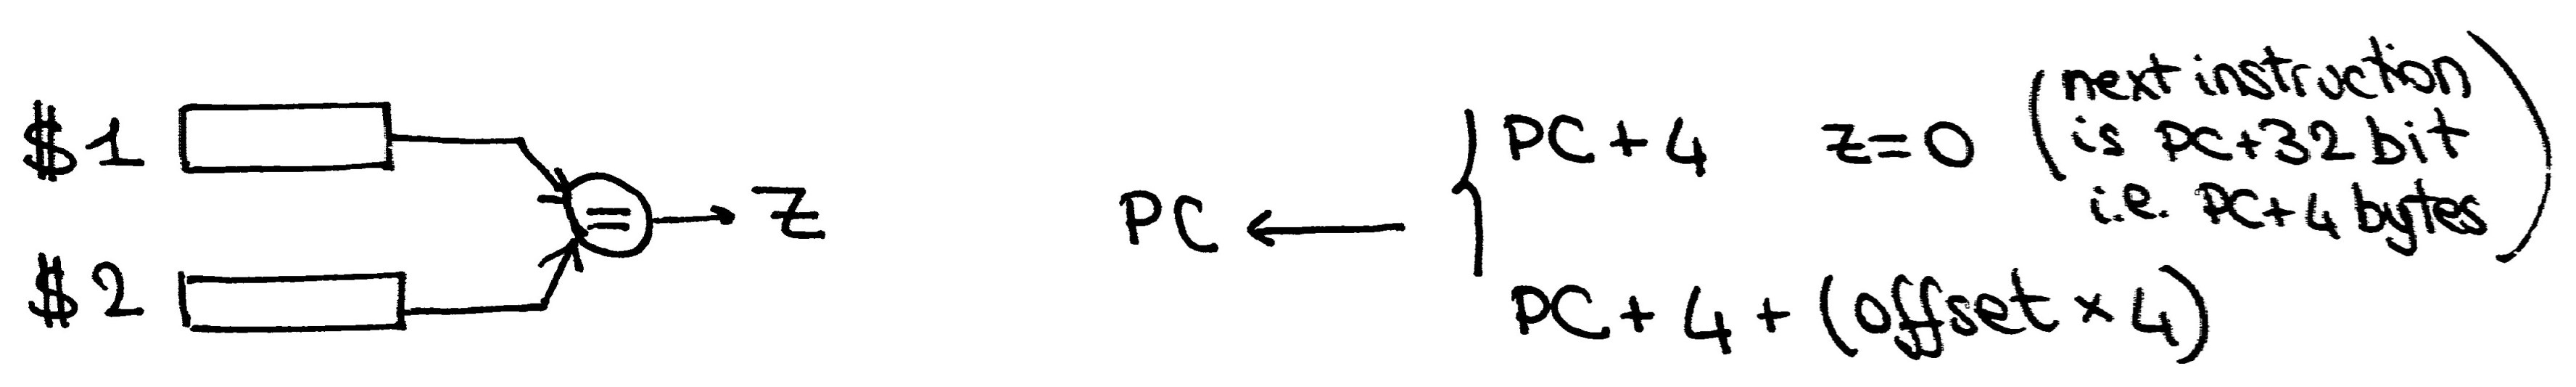
\includegraphics[width=0.85\linewidth]{img/img3/2}
    \end{center}
    Again the offset written in the instruction doesn't contain the two LSB
    since they are stucked at '00', moreover it is represented in 2's complement
    (backward or forward branch).
    \textit{Format:}
    \begin{verbatim}
    |opcode(6 bit)|R_s(5 bit)|r_t(5 bit)|offset(16 bit)|
    \end{verbatim}
\end{itemize}
%%%%%%%%%%%%%%%%%%%%%%%%%%%%%%%%%%%%%%%%%%%%%%%%%%%%%%%%%%%%%%%%%%%%%%%%%%%%%%%%
%%%%%%%%%%%%%%%%%%%%%%%%%%%%%%%%%%%%%%%%%%%%%%%%%%%%%%%%%%%%%%%%%%%%%%%%%%%%%%%%
%%%%%%%%%%%%%%%%%%%%%%%%%%%%%%%%%%%%%%%%%%%%%%%%%%%%%%%%%%%%%%%%%%%%%%%%%%%%%%%%
\subsection{Hardware architecture}
\subsubsection{Metrics}
The most important performance metric is \textit{execution time} which
corresponds to the amount of time required to perform a given set of
instructions. It can expressed as:
\begin{equation*}
T_{exec}= N_{instr} \cdot T_{cycle} \cdot CPI
\end{equation*}
Where:
\begin{itemize}
  \item $N_{instr}$ is the number of instructions to be executed, moreover we
    assume that every instruction takes the same amount of time to be completed.
  \item $T_{cycle}$ is the clock period which depends on the implementation
    technology and the hardware architecture.
  \item $CPI$ are the cycles per instruction, i.e. how many clock cycles we
    need for a single instruction.
\end{itemize}
In order to reduce $T_{exec}$ given $N_{instr}$ (related to a specific
application) we can decrease $T_{cycle}$ or $CPI$. Reducing $CPI$ probably means
to be able to perform more instructions in parallel, leading to the so called
parallel architecture; instead working on $T_{cycle}$ allows to achieve a faster
clock frequency. The second option can be exploited in two ways: improve
technology or having an architecture able to intrinsically proceed faster, that
is pipelinig since we divide the critical path and can achieve higher clock
frequency. MIPS exploits the basic idea of pipelining.
%%%%%%%%%%%%%%%%%%%%%%%%%%%%%%%%%%%%%%%%%%%%%%%%%%%%%%%%%%%%%%%%%%%%%%%%%%%%%%%%
%%%%%%%%%%%%%%%%%%%%%%%%%%%%%%%%%%%%%%%%%%%%%%%%%%%%%%%%%%%%%%%%%%%%%%%%%%%%%%%%
%%%%%%%%%%%%%%%%%%%%%%%%%%%%%%%%%%%%%%%%%%%%%%%%%%%%%%%%%%%%%%%%%%%%%%%%%%%%%%%%
\subsection{MIPS datapath}
\begin{center}
  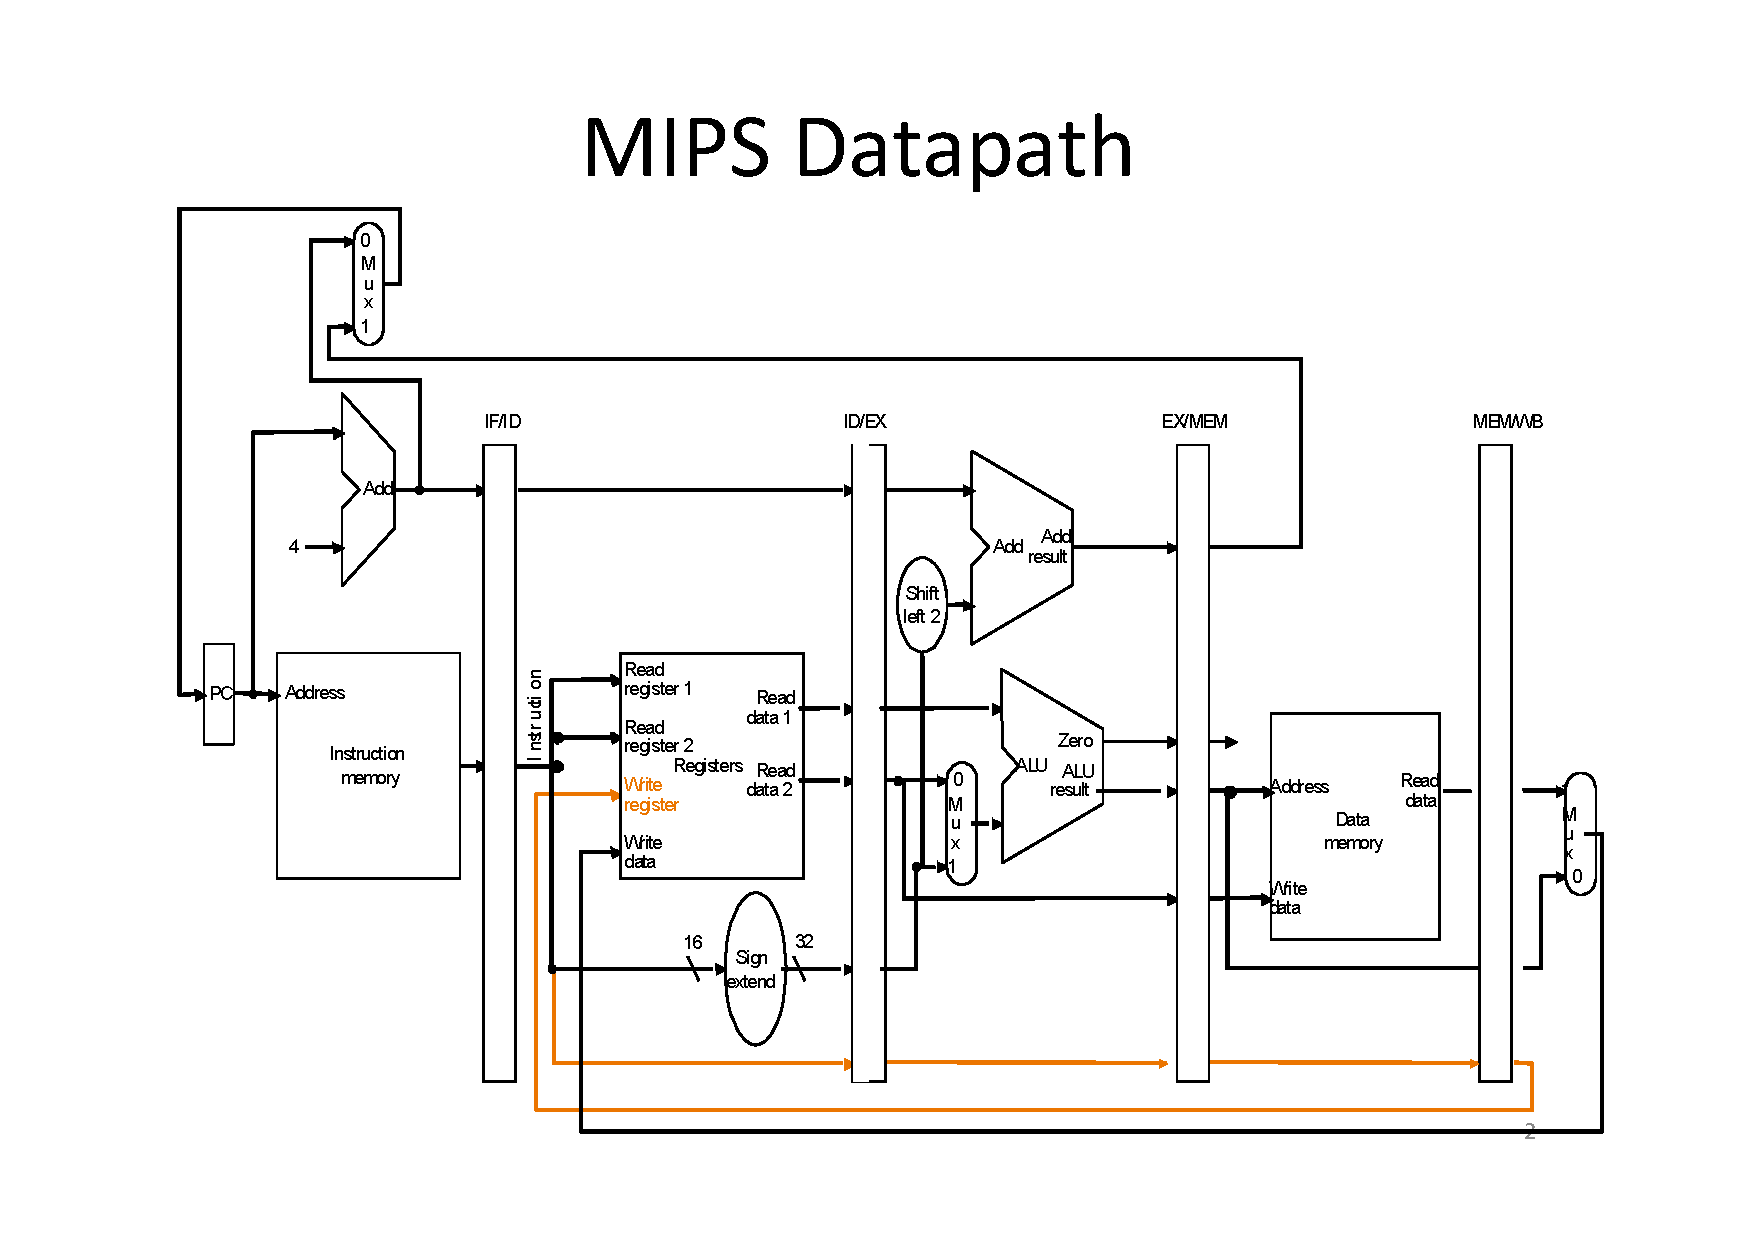
\includegraphics[width=1.0\linewidth]{img/img3/mips1}
\end{center}
There are many stages separated by pipelining registers, in this case 5
pipelining levels are presented. Looking at each step:
\subparagraph{Stage 1: Instruction fetch stage}
The purpose of this stage is to fetch instructions from the memory. Using this
organization two different memories are available, one for data and one for
instruction (so it is an Harvard architecture and not Van Neumann). Here there
is the program counter which provides the address related to the instruction to
be fetched and an adder which add +4 to the current PC (+4 means moving 4 bytes
forward, so to the next instruction); the updating of PC is performed using a
multiplexer (sequential or jump).\\
In every processor a fetch unit is needed, however it may be much more complex
than this one. For example in a parallel architecture (where we have to fetch
more than one instruction) if a jump occurs it may be very difficult manage it,
so in this case the stage is divided into smaller stages to keep high the clock
frequency.
\subparagraph{Stage 2: Instruction decode}
In this stage the instruction is decoded and a reading from RF is performed.
We assume that a multi port register file having 32 word (32 registers) is
employed meaning that we can read two data at the same time. To access the RF
2 source addresses are needed ($r_s, r_t$). In this stage we also perform the
decoding of the instruction. For these first two steps (fetch and read two
operands from RF) are always performed in order to avoid latency between the
instruction decoding and the RF access since no control signals are needed.\\
This means that the instruction decoding can be done in parallel to the RF
access so that at the following step we already have the data and the control
signals ready to be used.
\subparagraph{Stage 3: execution stage}
Here the actual computation is performed; the ALU is the kernel and it is able
to perform integer operation (surely ADD, SUB; MPY may required external unit),
it receives two operands taken from the pipeline registers or from the register
file directly. However we may need to follow a different path for instance to
perform \verb|lw $2, 20($1)| since the second operand (offset) has to be taken
directly from the instruction: we need to select the correct source for ALU
inputs.\\
In this scheme there is also an upper adder: it is not a complete ALU but it is
an extra hardware employed in branch operations. In this particular case the
comparison is done by the ALU (like \verb|beq|) but in parallel we have to
prepare the address at which jump if the branch has to be performed. This
required to compute $4 \cdot offset + PC+4$ but this cannot be done by ALU
since it is already busied by the comparison, meaning that we required some
extra-hardware (i.e. upper adder).
\subparagraph{Stage 4: Data memory}
This stage is only used if we have to perform a memory instruction. Usually the
address is coming from the ALU (so in the previous step ALU computes the address
of the memory as base address plus offset), then we need a write port (to store
a data) or a read port. We assume that the memory can only perform either a
write either a read.
\subparagraph{Stage 5: Write back}
We may have to process the data coming out from the memory or from the ALU, so
we have to store the result of the ALU or the data read from the memory into the
register file, meaning that the output of the multiplexer comes back into the
write port of the register file.
%%%%%%%%%%%%%%%%%%%%%%%%%%%%%%%%%%%%%%%%%%%%%%%%%%%%%%%%%%%%%%%%%%%%%%%%%%%%%%%%
%%%%%%%%%%%%%%%%%%%%%%%%%%%%%%%%%%%%%%%%%%%%%%%%%%%%%%%%%%%%%%%%%%%%%%%%%%%%%%%%
%%%%%%%%%%%%%%%%%%%%%%%%%%%%%%%%%%%%%%%%%%%%%%%%%%%%%%%%%%%%%%%%%%%%%%%%%%%%%%%%
\subsection{MIPS datapath with control signals}
In this scheme the same informations as before with control signals are
reported, the control unit is actually the decoding unit which takes part of the
instruction as an input and generates three different outputs divided as
follows: WB, M an EX. Each of them contains all the control signals generated in
step 2 but that are related to the following steps, meaning that in the EX field
there are all the controls signal required in the execution stage, in M the ones
required in the memory (so it has to be delayed), and in WB  the ones for the
fifth stage.\\
\textit{Issue}:data and control signal have to be delayed of the same amount in
order to guarantee coherence.
\begin{center}
  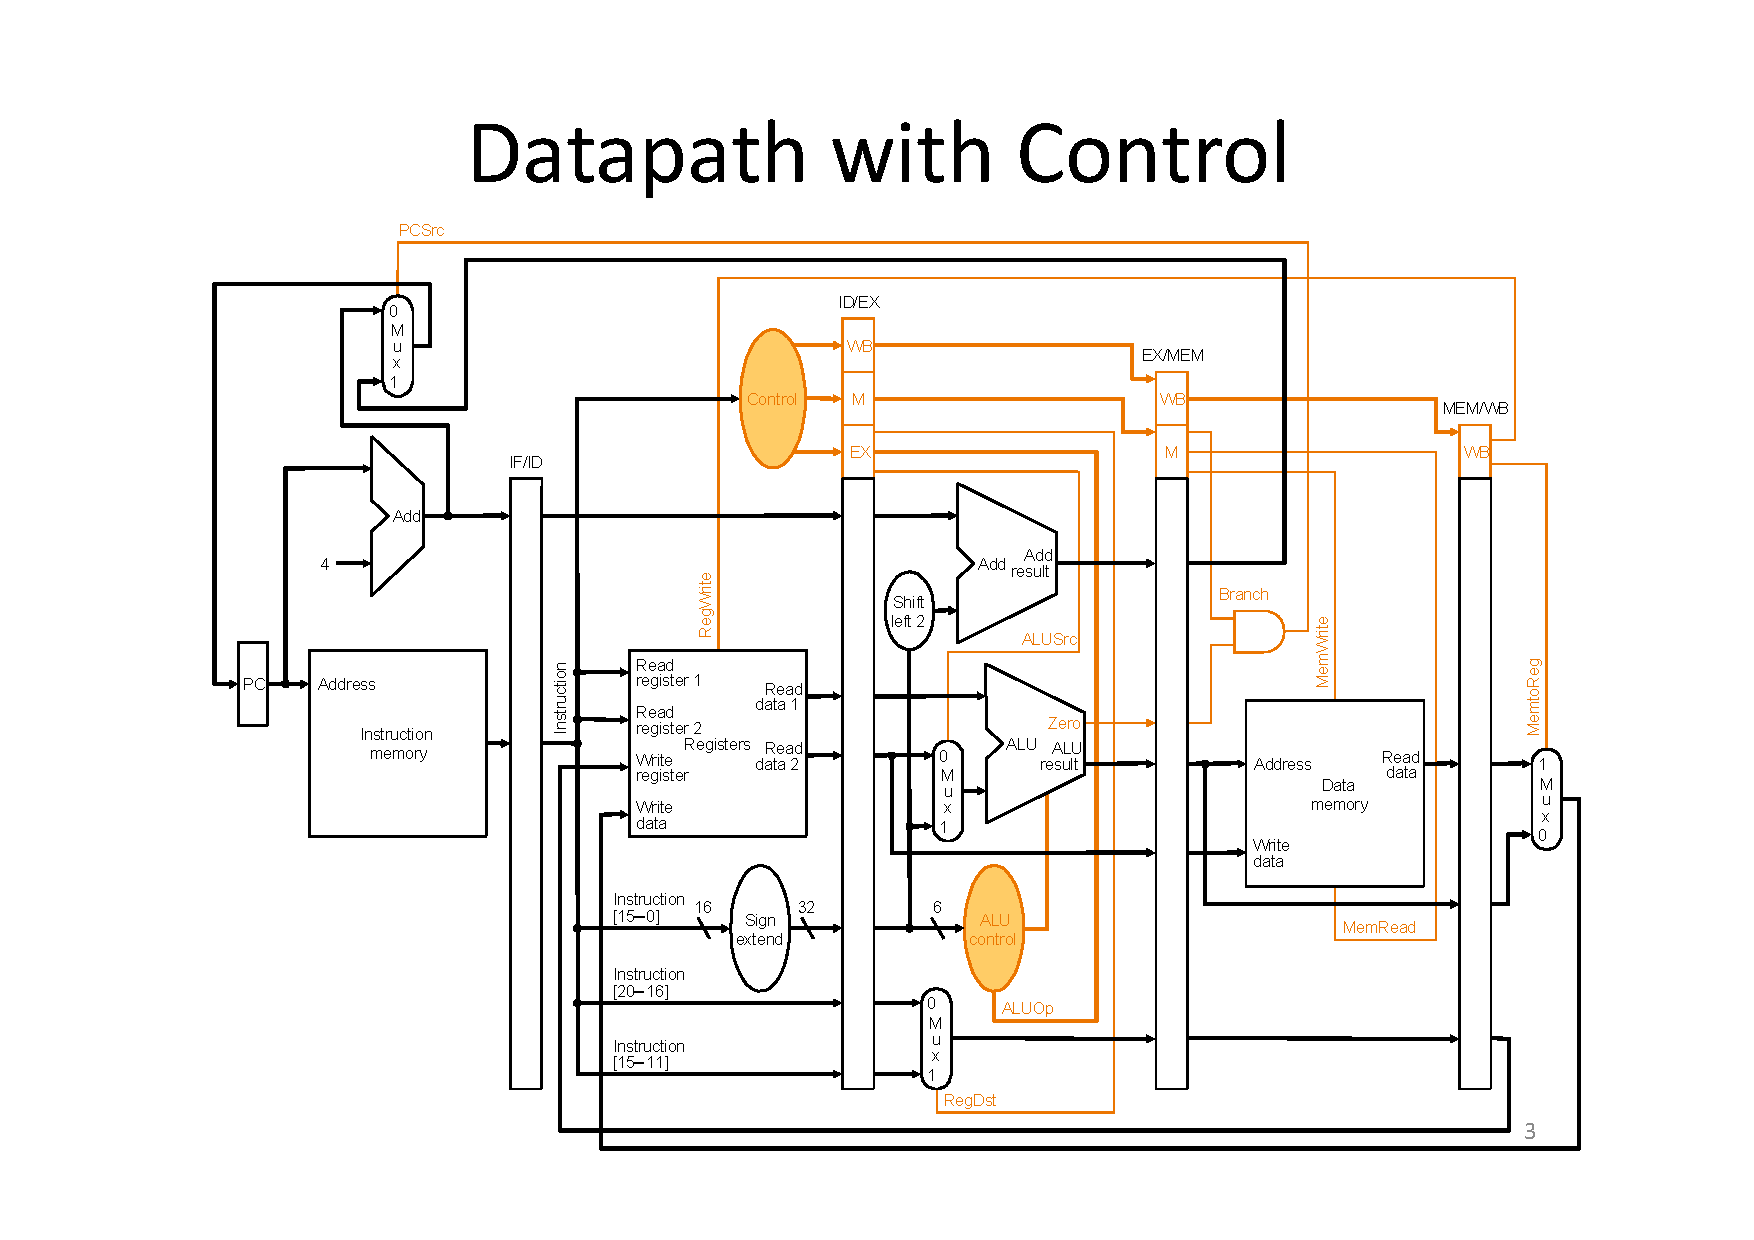
\includegraphics[width=1.0\linewidth]{img/img3/mips2}
\end{center}
\section{Hazards}
A pipelined organization of the processor guarantees a high throughput, however
we have to analyze how hazards are generated and how handled them. Hazards can
be divided into:
\begin{itemize}
  \item Structural hazards.
  \item Data hazards.
  \item Control hazards.
\end{itemize}
%%%%%%%%%%%%%%%%%%%%%%%%%%%%%%%%%%%%%%%%%%%%%%%%%%%%%%%%%%%%%%%%%%%%%%%%%%%%%%%%
%%%%%%%%%%%%%%%%%%%%%%%%%%%%%%%%%%%%%%%%%%%%%%%%%%%%%%%%%%%%%%%%%%%%%%%%%%%%%%%%
%%%%%%%%%%%%%%%%%%%%%%%%%%%%%%%%%%%%%%%%%%%%%%%%%%%%%%%%%%%%%%%%%%%%%%%%%%%%%%%%
\subsection{Structural hazards}
A structural hazard occurs when there's a conflict on the use of a piece of
hardware. For instance:
\begin{verbatim}
    C1  C2  C3  C4  C5  C6  C7
--------------------------------
I1| IF  D   EX  M   WB
I2| -   IF  D   EX  M   WB
I3| -   -   IF  D   EX  M   WB
I4| -   -   -   IF  D   EX
\end{verbatim}
This is a typical instructions flow with no branches; let's consider instruction
I1 and I4 in cycle number 4 (C4), here we have for I1 the memory stage and for
I4 the instruction fetch: if we are using a Von Neumann architecture (where
there is no separation between data memory and instruction memory) we cannot
perform a write and a read in the memory at the same time. There is no solution
for this kind of hazard, to avoid them we have to design the proper ISA and
architecture.\\
Another kind of conflict is reported in cycle 5: both I1 and I4 instructions are
trying to access the Register File (I4 reads from the RF while I1 has to perform
a write back).  Potentially this is a second example of structural hazard.
However RF is usually dersigned in order to allow 2 read and one write operation
in the same cycle (having distinct ports for each op).
Structural hazard is more frequent in superscalar architectures.
%%%%%%%%%%%%%%%%%%%%%%%%%%%%%%%%%%%%%%%%%%%%%%%%%%%%%%%%%%%%%%%%%%%%%%%%%%%%%%%%
%%%%%%%%%%%%%%%%%%%%%%%%%%%%%%%%%%%%%%%%%%%%%%%%%%%%%%%%%%%%%%%%%%%%%%%%%%%%%%%%
%%%%%%%%%%%%%%%%%%%%%%%%%%%%%%%%%%%%%%%%%%%%%%%%%%%%%%%%%%%%%%%%%%%%%%%%%%%%%%%%
\subsection{Data hazards}
Data hazards occur when instructions that exhibit data dependence modify data in
different stages of a pipeline. Ignoring potential data hazards can result in
race conditions (also termed race hazards). There are three situations in which
a data hazard can occur:
\begin{itemize}
  \item \textbf{RAW} read after write (true dependency)
  \item \textbf{WAR} write after read (anti-sependency)
  \item \textbf{WAW} write after write (output dependency)
\end{itemize}
\subsubsection{WAR}
(i2 tries to write a destination before it is read by i1) A write after read
(WAR) data hazard represents a problem with concurrent execution.
\begin{verbatim}
  I1:add  R4  R1  R3      R4 <- R1 + R3 // R1 is source reg
  I2:add  R4  R1  R5      R4 <- R1 + R5 // R1 is source reg
\end{verbatim}
In any situation with a chance that i2 may finish before i1 (i.e., with
concurrent execution), it must be ensured that the result of register R5 is not
stored before i1 has had a chance to fetch the operands.
\subsubsection{WAW}
(i2 tries to write an operand before it is written by i1) A
write after write (WAW) data hazard may occur in a concurrent execution
environment.
\begin{verbatim}
  I1:add  R2  R4  R7      R2 <- R4 + R7 // R2 is dest reg
  I2:add  R2  R1  R3      R2 <- R1 + R3 // R2 is dest reg
\end{verbatim}
The write back (WB) of i2 must be delayed until i1 finishes executing.
\subsubsection{RAW}
(i2 tries to read a source before i1 writes to it) A read after write (RAW) data
hazard refers to a situation where an instruction refers to a result that has
not yet been calculated or retrieved. This can occur because even though an
instruction is executed after a prior instruction, the prior instruction has
been processed only partly through the pipeline.
\begin{verbatim}
  I1:add  R2  R1  R3      R2 <- R1 + R3 // R2 is dest reg
  I2:add  R4  R2  R5      R4 <- R2 + R5 // R2 is source reg
\end{verbatim}
The first instruction is calculating a value to be saved in register R2, and the
second is going to use this value to compute a result for register R4. However,
in pipelined architecture the second instruction is started just one cycle after
the first one:
\begin{verbatim}
  C1  C2  C3  C4  C5  C6
---------------------------
I1| IF  D EX  M WB
I2| -   IF  D   EX  M   WB
\end{verbatim}
Only at the end of $5^{th}$ cycle the result of \verb|R1+R3| is available in
\verb|R2|, however we would like to read it in the decode stage of the second
instruction, i.e. in $3^{rd}$ clock cycle. This problem comes from the
pipelining organization, \textit{longer is the pipeline higher is the
possibility to have problems like this}. Many solutions may handle this
conflict:
\begin{itemize}
  \item Stall.
  \item Scheduling at compiler level.
  \item Forwarding/bypassing.
\end{itemize}
\subsubsection{Stall}
  A stall means having the pipeline frozen for one or more clock cycles in order
  to wait the data dependency to be propagated. The basic idea is to insert two
  NOP instructions between I1 and I4 to have no more conflict, so that all data
  will be frozen. However to avoid the conflict we have to wait, the instruction
  time will increase and there are a lot of situations where this data
  dependency can occur.
\subsubsection{ReScheduling}
   A compiler/assembler translates assembly language into binary code to be
   downloaded into the instruction memory. By doing that, the compiler may be
   asked to perform some optimizations like finding data hazard instruction and
   insert between them some other useful instructions while avoiding data
   dependencies. If this \textit{rescheduling} is not possible the compiler will insert
   NOPs; there is no guarantee to find a proper rescheduling.
  % \subparagraph{Example}
  % The starting code is:
  % \begin{verbatim}
  % a=b+c
  % d=e-f
  % \end{verbatim}
  % which is translated into assembler (always before the load in registers and
  % then the arithmetic operation):

  % \begin{verbatim}
  % lw R1, b
  % lw R2, c
  % ...
  % \end{verbatim}
  % Potentially we may have data dependencies since the second and the third are
  % two following instructions and we already know that when \verb|c| is required
  % in the third operation it is still not present in the register. A similar
  % situation is hiring for the $6^{th}$ and $7^{th}$ instructions. As an
  % alternative approach the compiler may be required to recognize this situation
  % and avoid the insertion of nop operations. In this particular case the load
  % for the second arithmetic operation has been allocated before the add
  % instruction.

  % \begin{verbatim}

  % ... new code...

  % \end{verbatim}

  % Similarly the storing of \verb|a| can keep separate the load of \verb|f| from
  % its usage, in this way there is no need to stall the processor.
\subsubsection{Forwarding/bypassing}
\begin{center}
  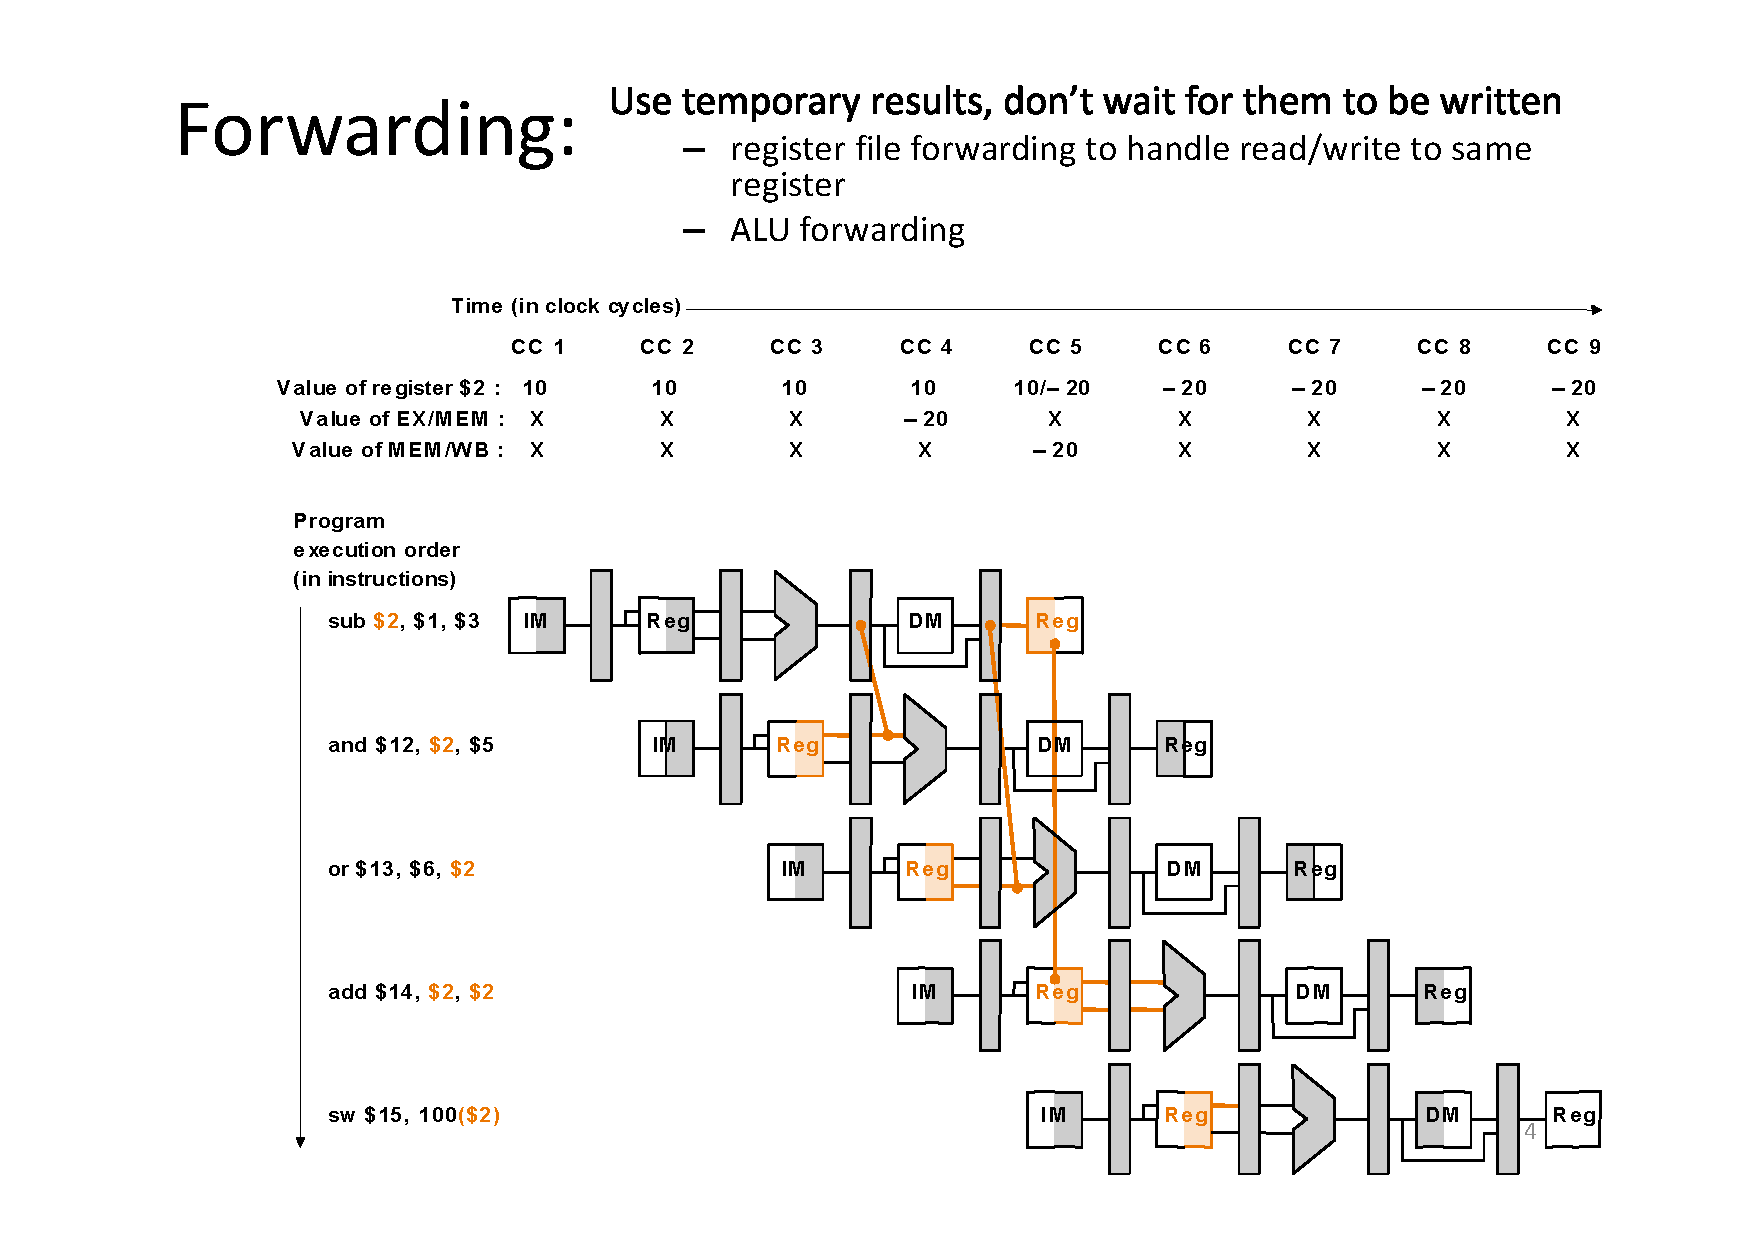
\includegraphics[width=1.0\linewidth]{img/img3/mips3}
\end{center}
In this sequence of instructions \$2 is the destination register of the first
operation while in all subsequent instructions it appears as source register.
At which stage we have the data ready to be written in RF \$2? At the end of
third cycle we already have the value which will be later written in \$2 so
actually the data itself is already available. The second operation cannot read
at the third cycle this data from RF, however in addition to save the first
operation result in RF we can forward it to the ALU for the second instruction
(I2/EX). This kind of bypass takes an output of ALU and put it back at ALU
input. Looking at the previous graph this operation is like a forward operation,
however since there is only one ALU it is a bypass (from the hardware point of
view). This means that we need to insert some multiplexers at the input of the
ALU, but it is a more than reasonable solution. Same thing occurs for the other
operations.
\begin{center}
  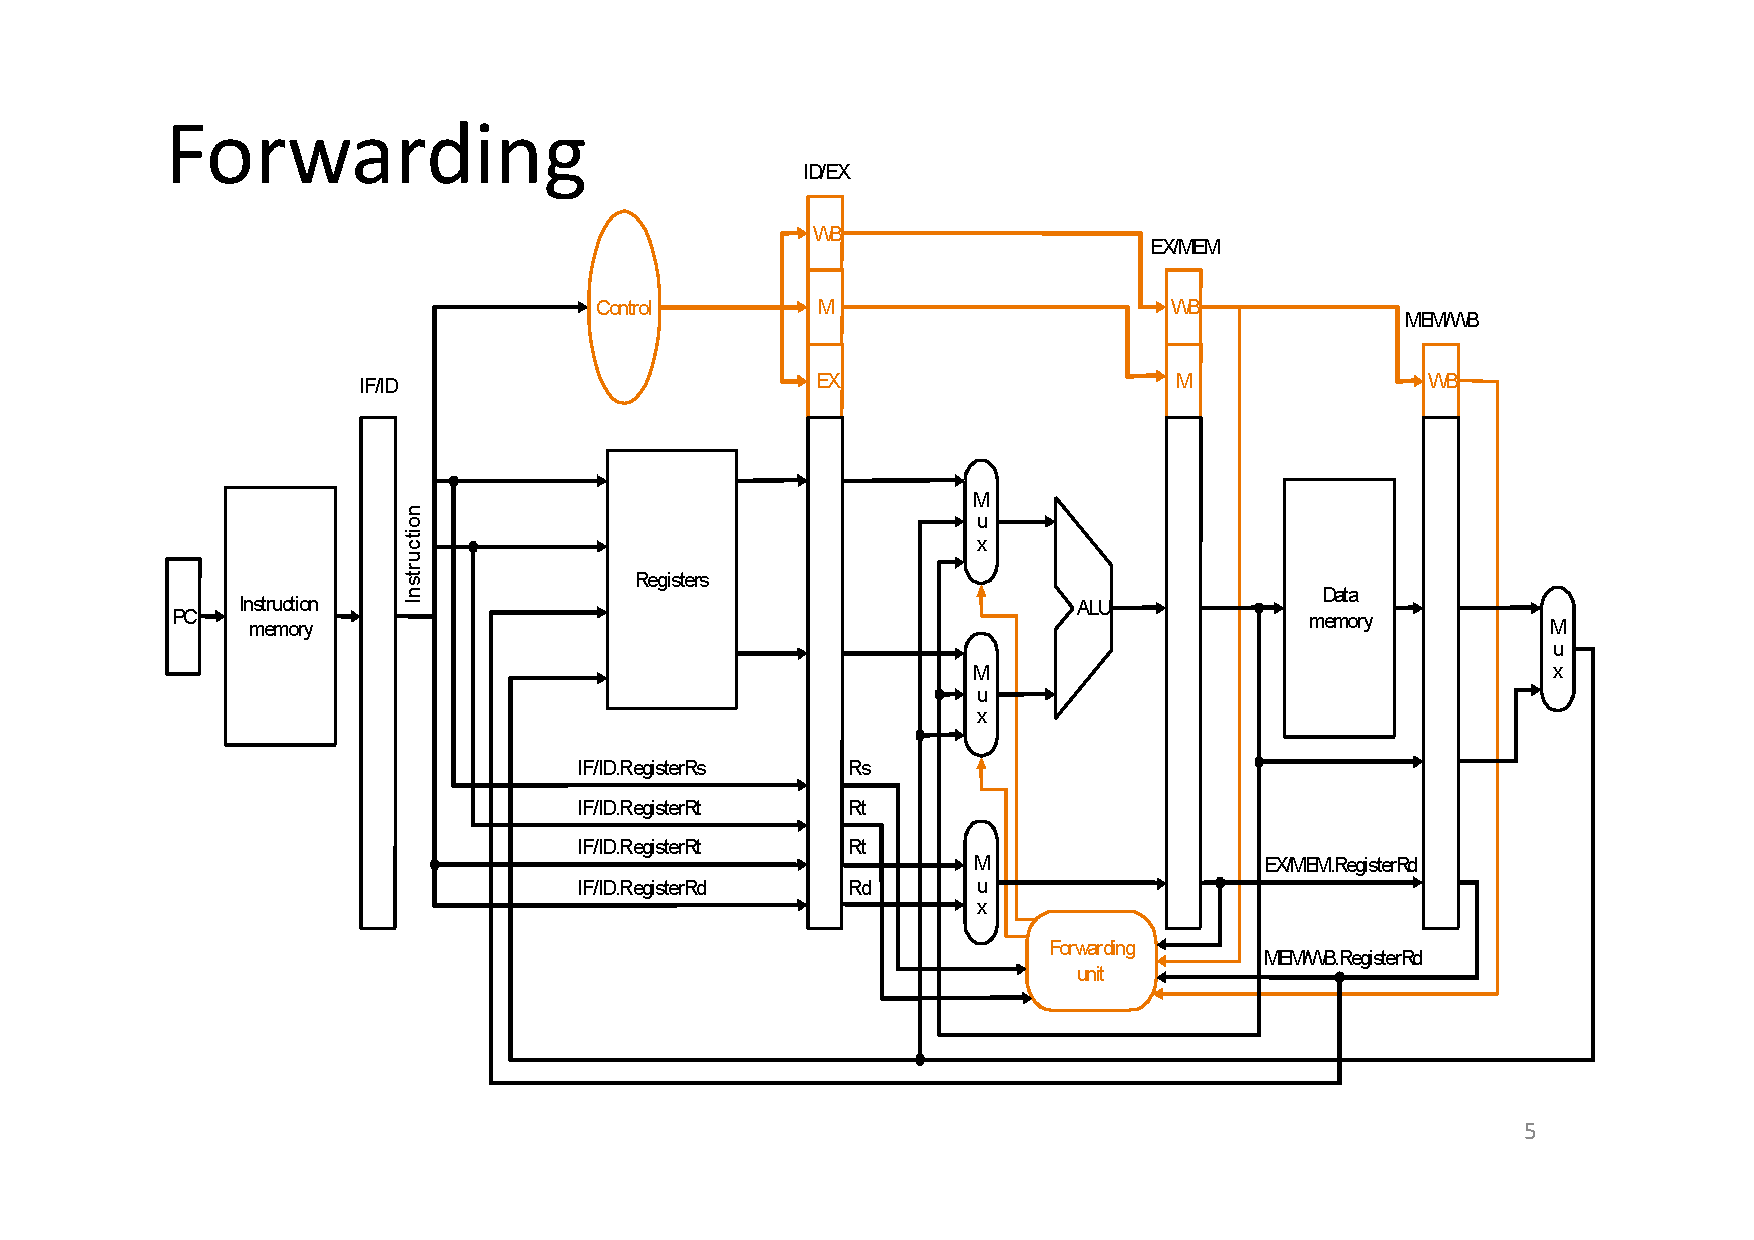
\includegraphics[width=0.8\linewidth]{img/img3/mips4}
\end{center}
The scheduling solution maybe of some help but it doesn't guarantee success.
Regarding the forwarding approach, actually we need more than one kind of
bypass.\\
ALU has to been provided by two multiplexers, whose inputs may be: RF output,
value stored in EX Pipeline register, value stored in DATA STORE pipeline
(forwarding of 1 or 2 stages).\\
If the pipeline is longer, we may need a forwarding up to 4-5-6 stages. The
selection signals for the multiplexers are provided by the forwarding unit
starting from the comparison between registers involved in close instructions
(meaning $R_s$ and $R_t$ which are currently starting the EX stage, $R_d$ for
the instruction in the memory stage and $R_d$ just out the EX stage), moreover
it receives also some control signals since it is not sufficient to look at
the address registers. An example of the algorithm to be employed is the
following:
\begin{verbatim}
// if we have to write smtg in RF, so a data hazard may occour
if(EX/MEM.regWrite)
  // location 0 in RF usually contains constant (like all 0)
  if(EX/MEM.Rd =! 0)
    //compare destination and source registers for different instructions
    if(EX/MEM.Rd == ID/EX.Rs)
      // in case of same name do forwarding from EX/MEM to ID/EX
      ForwardA=10;
\end{verbatim}
Recall that multiple forwarding at the same time are possible (i.e. a value in
reg MEM/WB is needed both by ID/EX and EX/MEM at the same cycle), hence it is
rather a complex unit. The complexity grows quadratically with respect to the
numbert of paths that are possible to take by the forwarding mechanism.
\begin{center}
  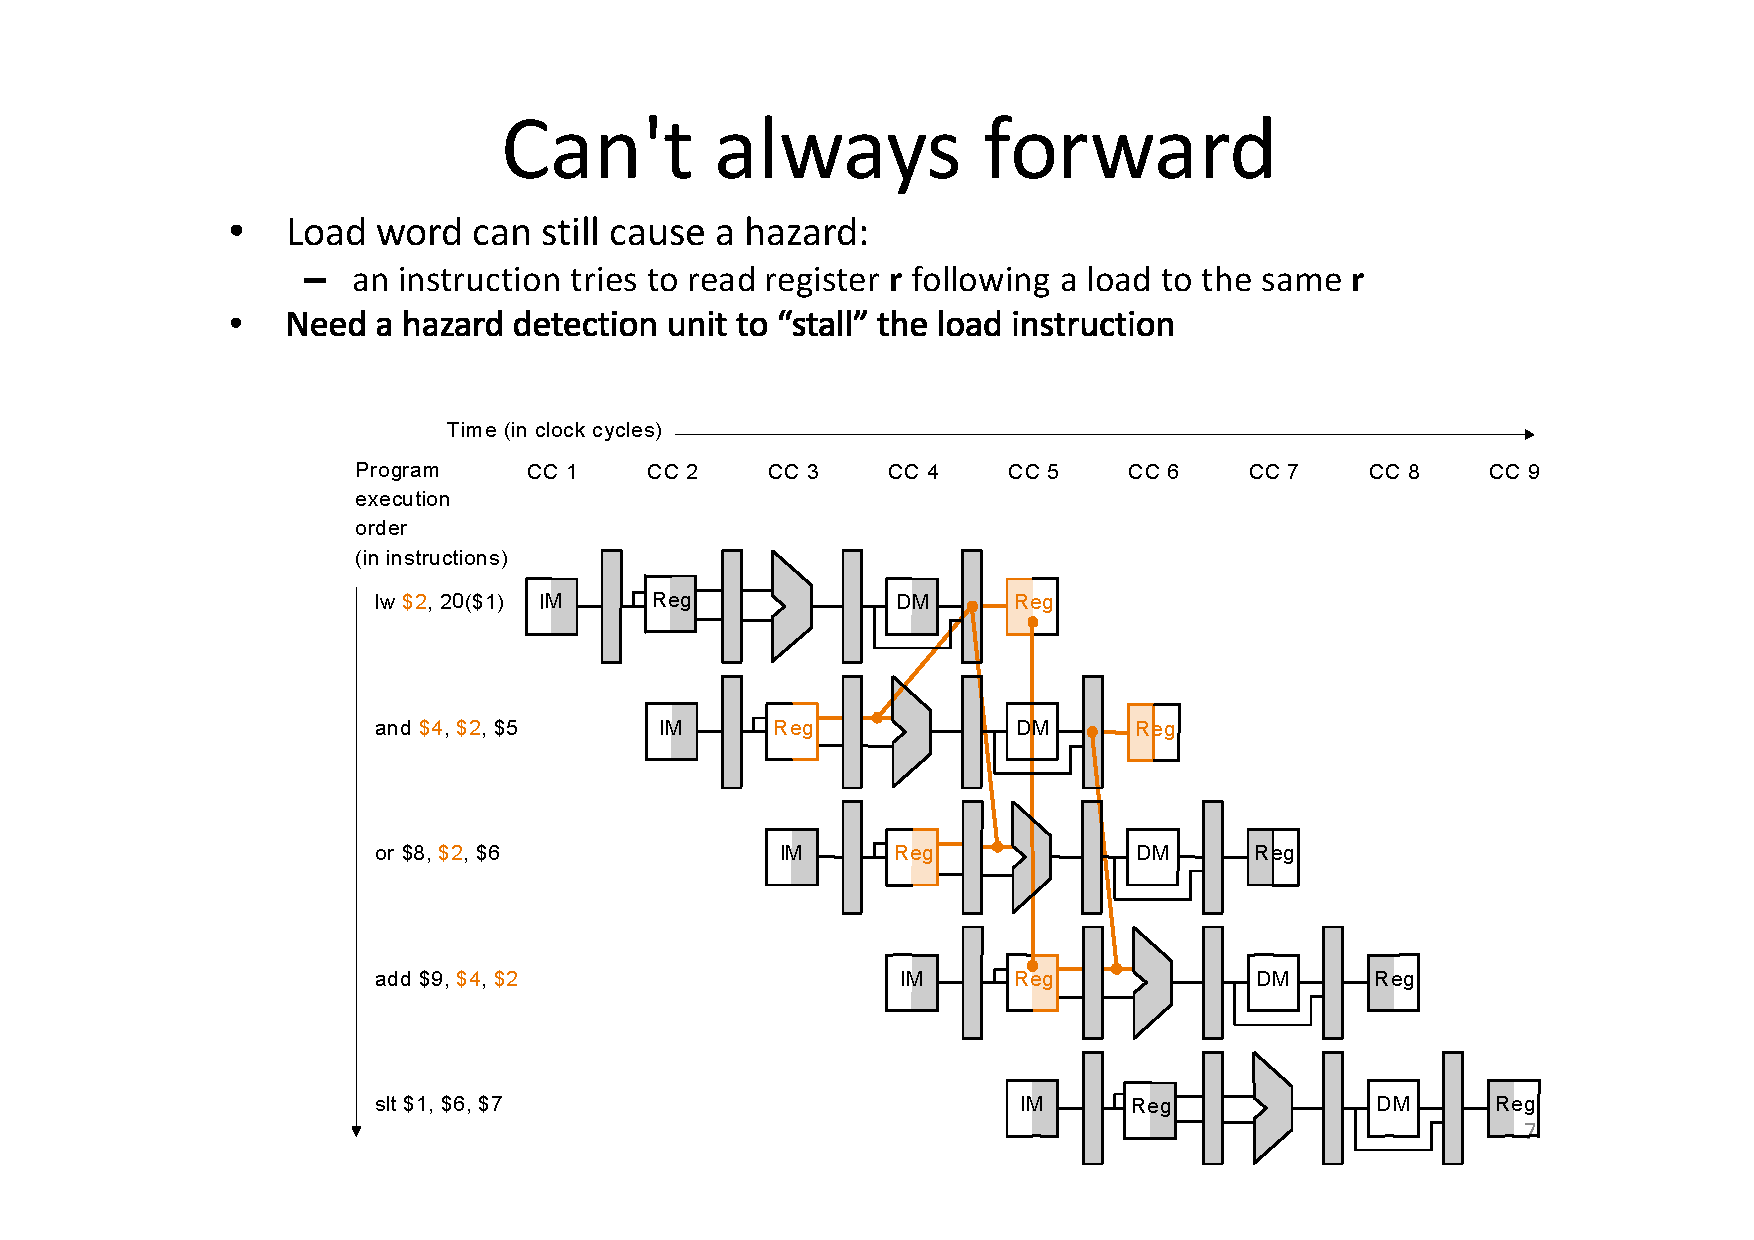
\includegraphics[width=1.0\linewidth]{img/img3/mips5}
\end{center}
\textit{Forwarding can not go back in time}.\\
There are situations where forwarding does not solve the problem.\\ For example,
when we have \verb|lw \$2, 20(\$1)| and then ther are many instructions with
source register \$2. This is a completely different situation since the first
instruction it is a \verb|lw|; we cannot perform a forwarding from the out of
Data Memory to the input of ALU since we generate the data at the end of forth
clock cycle but we need it at the beginning of the same cycle.  In fact the
direction of the arrow is coming back, meaning that we would need to perform a
forwarding back in time.  The idea is to mix forwarding with rescheduling (e.g.
swapping I2 with I3) so that we can perform a phys-able forward. If no
rescheduling is possible, a stall will be activate.\\
We both need a detection unit to find this situation and a mechanism to
generate a stall condition.
\begin{center}
  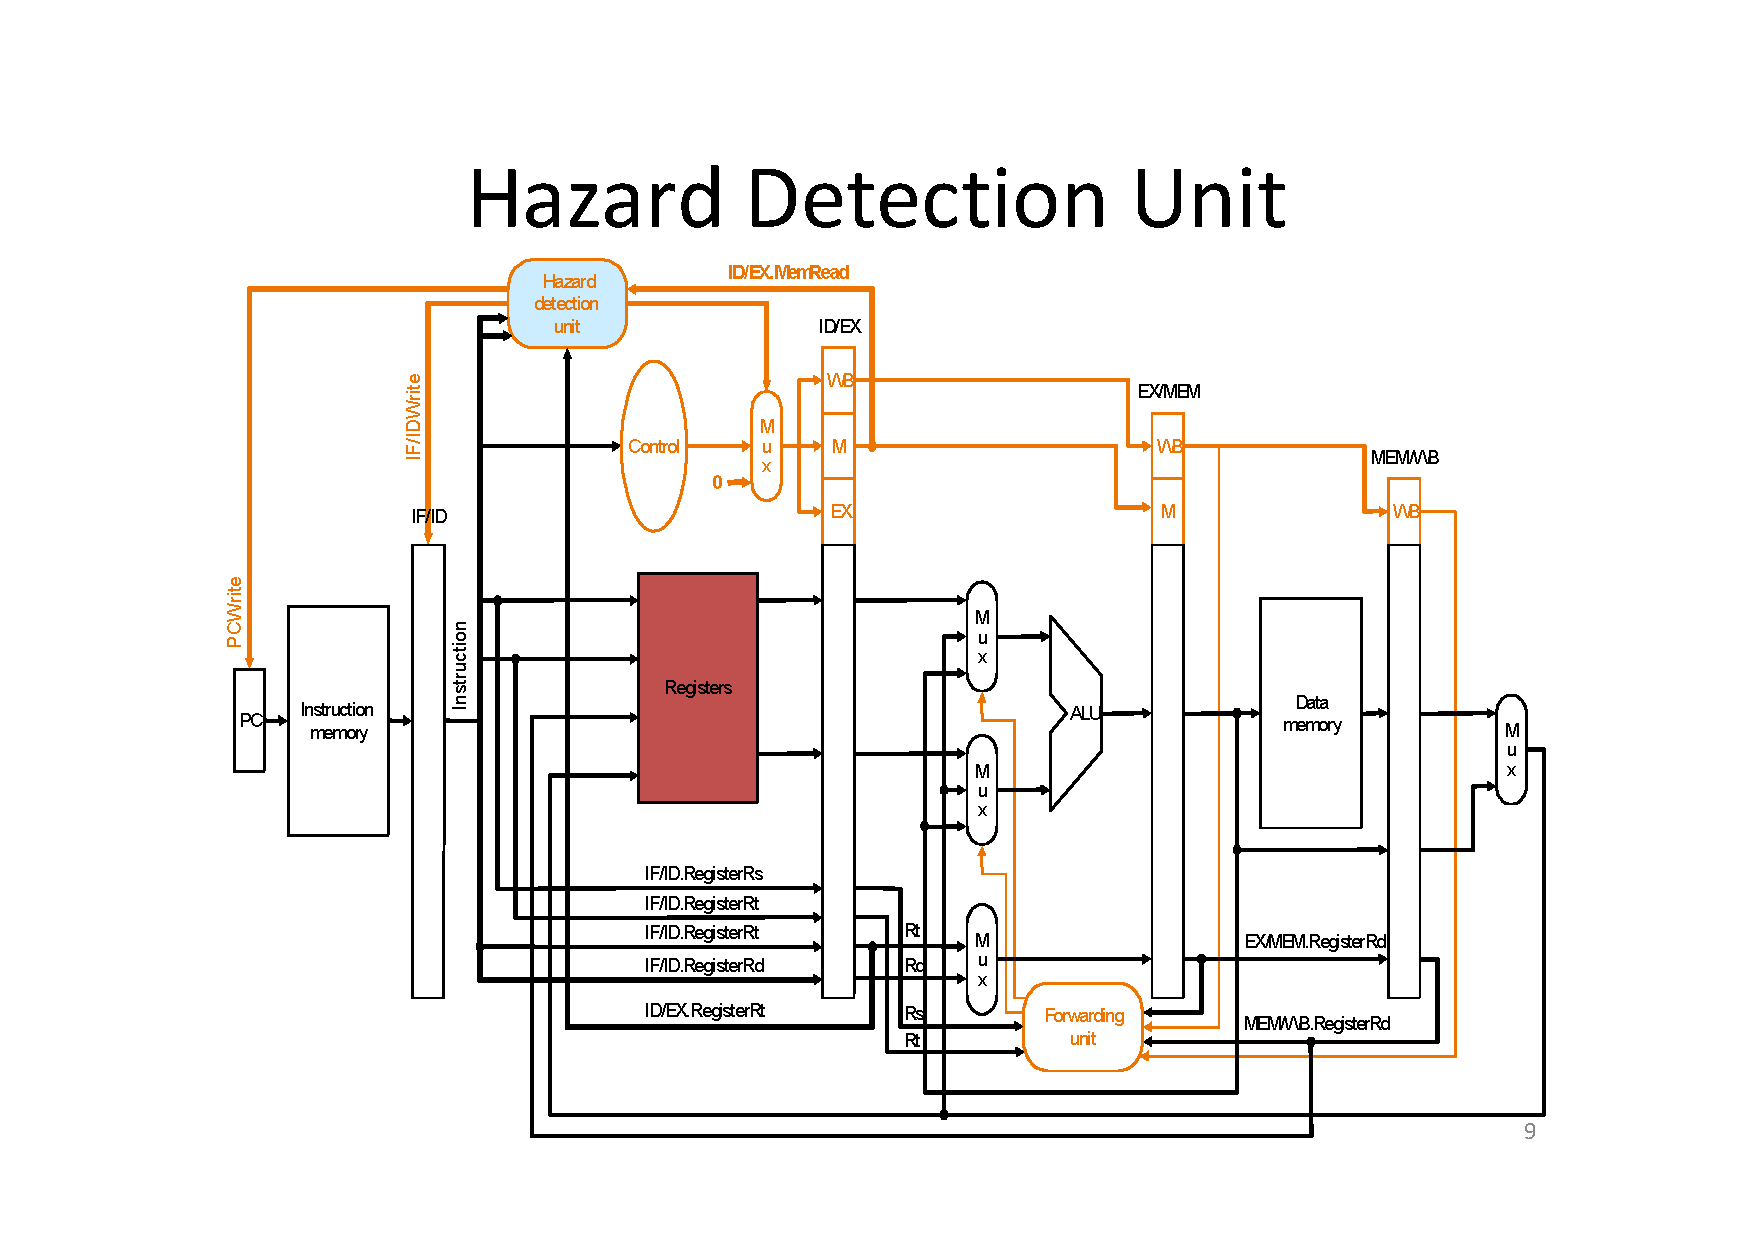
\includegraphics[width=1.0\linewidth]{img/img3/mips7}
\end{center}
In this architecture at the second stage additional element are added: an
\textbf{hazard detection unit} (inputs are registers and opcode) and a
\textbf{multiplexer} (inputs are \textit{control unit} result and a
\textit{string of zeros}). If an hazard situation is detected a NOP is inserted
and each stage will be frozen, just like a bubble that propagates to let other
operations proceeding and removing the conflicts. For MIPS this extra hardware
is relatively simple.\\The processor must be able to dynamically insert NOP if
required, but it has to work with a compiler which is able to perform the
scheduling.
%%%%%%%%%%%%%%%%%%%%%%%%%%%%%%%%%%%%%%%%%%%%%%%%%%%%%%%%%%%%%%%%%%%%%%%%%%%%%%%%
%%%%%%%%%%%%%%%%%%%%%%%%%%%%%%%%%%%%%%%%%%%%%%%%%%%%%%%%%%%%%%%%%%%%%%%%%%%%%%%%
%%%%%%%%%%%%%%%%%%%%%%%%%%%%%%%%%%%%%%%%%%%%%%%%%%%%%%%%%%%%%%%%%%%%%%%%%%%%%%%%
\subsection{Control hazards}
Control hazard may occur every time we have a deviation from the sequential
flow, since we may have problems with the pipeline. This situation is generated
by branch, jump, call to subroutine, exception (software call associated to a
particular problem), interrupts.
\begin{center}
  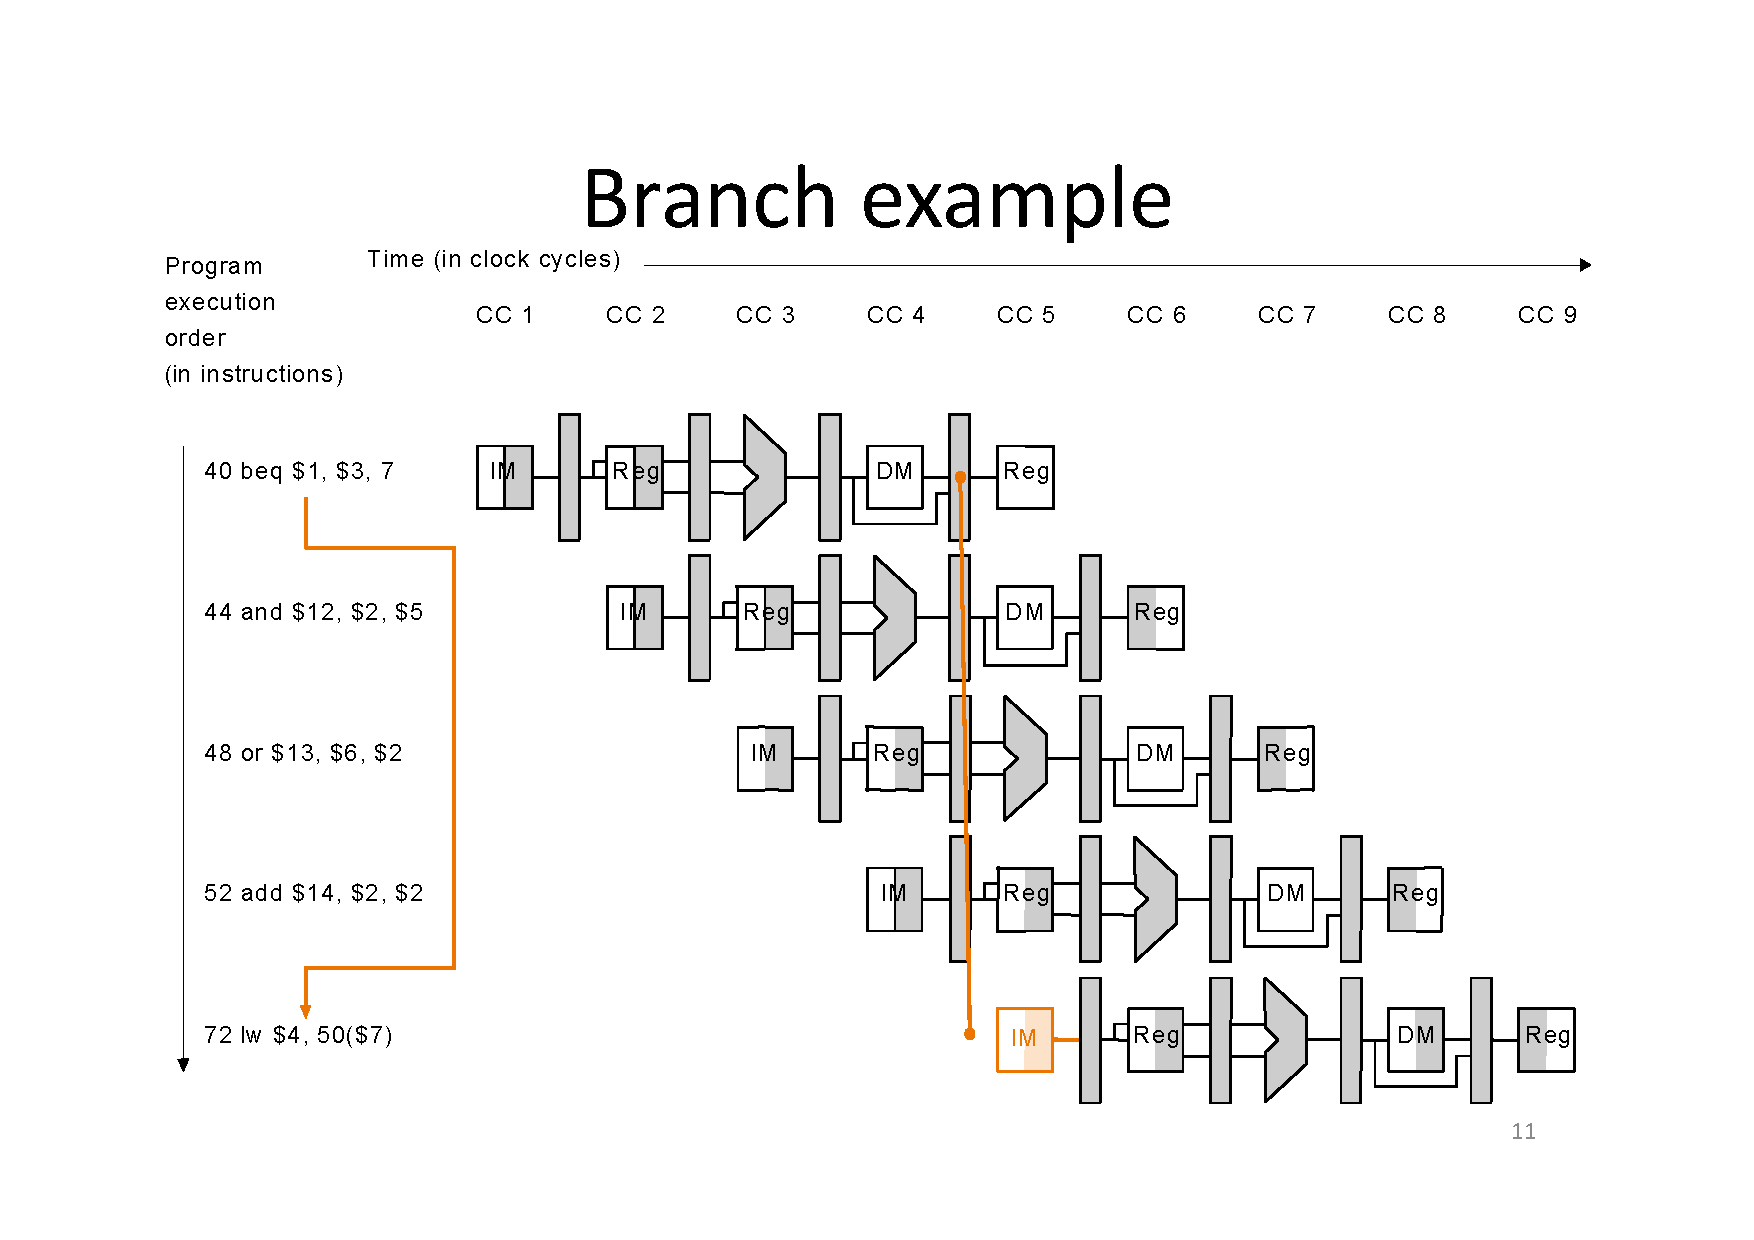
\includegraphics[width=0.9\linewidth]{img/img3/mips8}
\end{center}
\begin{center}
  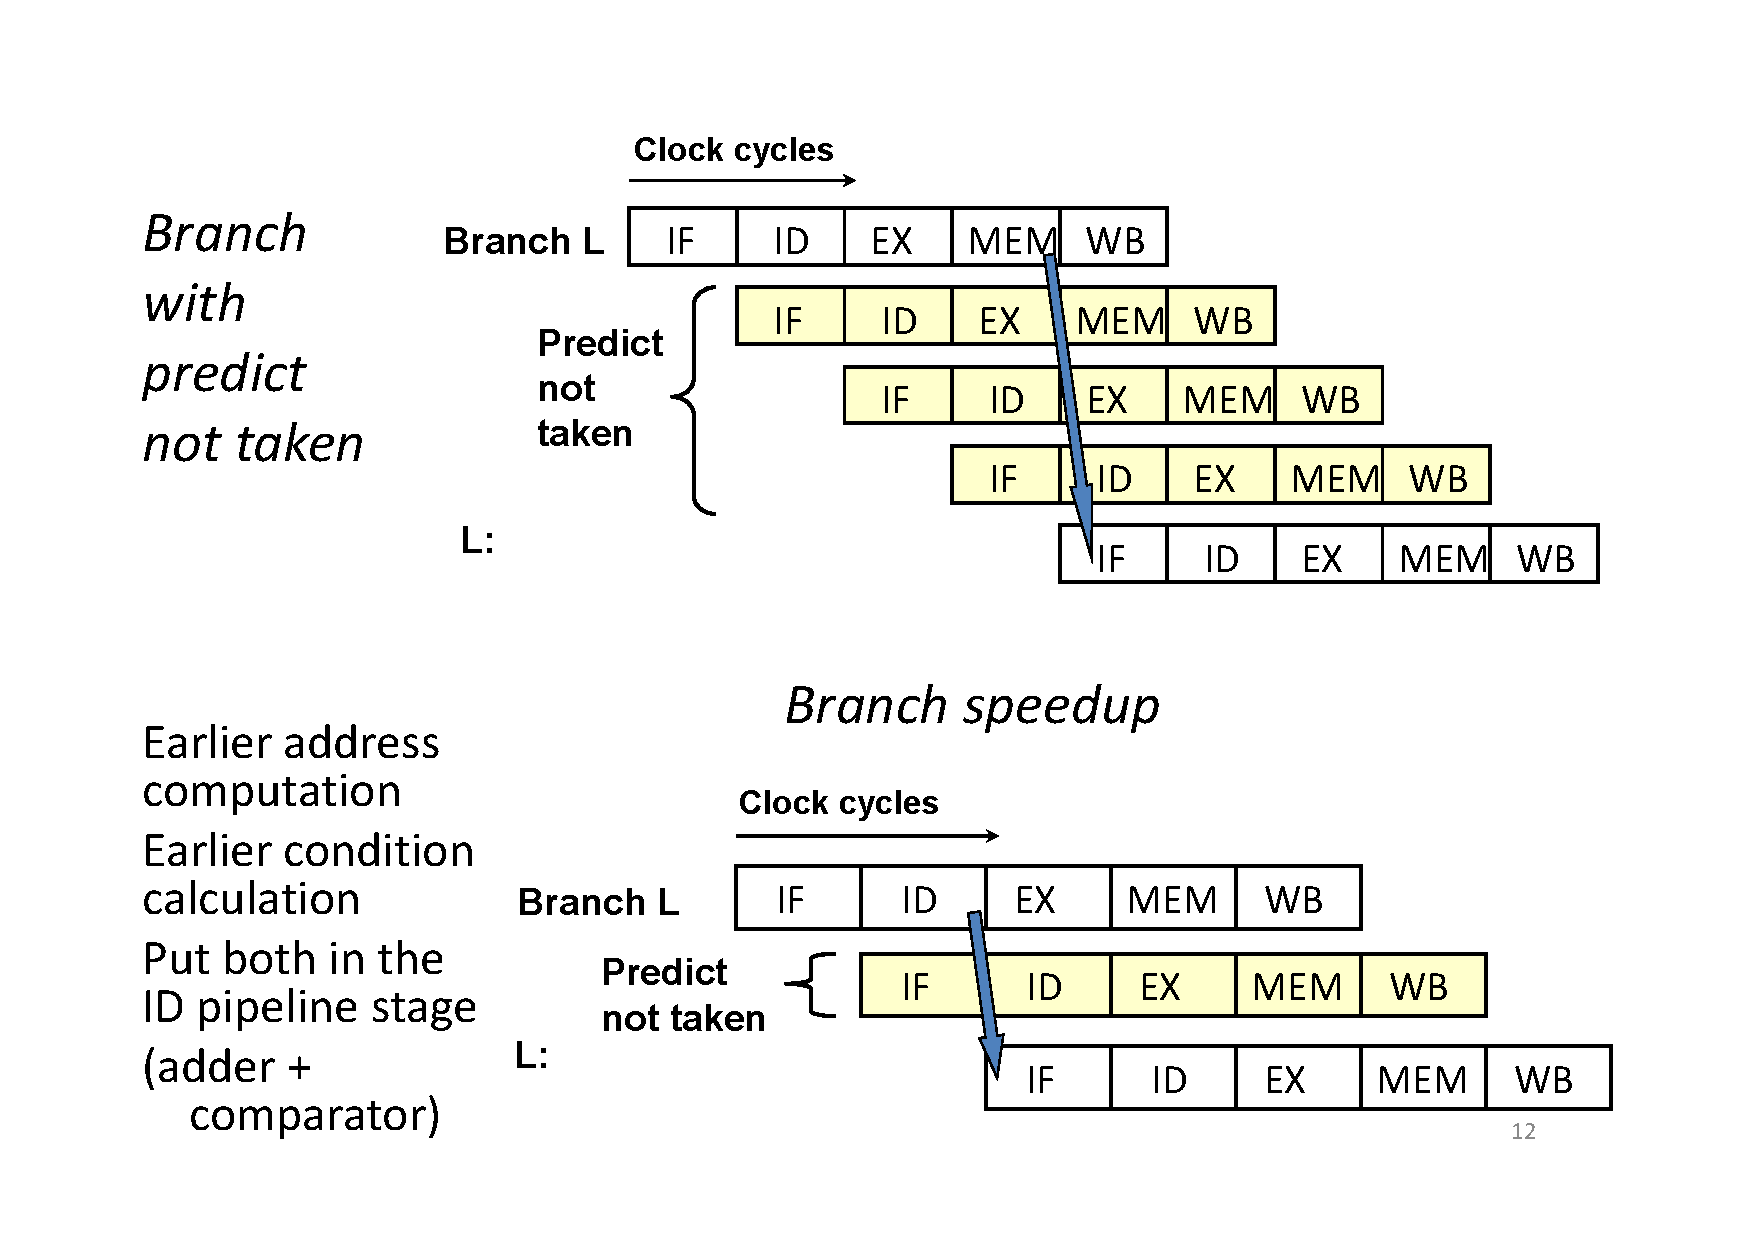
\includegraphics[width=0.9\linewidth]{img/img3/mips9}
\end{center}
If the branch is not taken the flow is sequential, otherwise we have to jump to
L. The point is that the decision requires time since it is needed to make a
comparison and to compute the target address (i.e. base address + offset for
the jump). As a consequence, we can be sure about the direction of the jump
only at the end of memory stage (for the branch instruction).\\In the execution
stage the ALU is performing the comparison (e.g. \verb|beq|) and the secondary
unit is performing the sum between base register and offset. This means that
both results (z flag and address result) needed to switch the multiplexer in
the first stage (which loads the proper PC) are ready only in memory stage. As
a consequence, only at the end of memory stage the correct PC for the
following instruction is set. Since all these operations take place, 4
instructions will be fetched, inserted into the pipeline and partially
performed.\\
Making a wrong prediction implies having a penalty of three cycles, since the
partially performed instruction must be throwed away. Something can be improved
by allocating some more hardware resources. There are a numbers of possible
solutions:
\begin{itemize}
  \item \textbf{Improved decode stage}: moves the branch verification from ther
    EX to D stage. Of course we cannot perform it in F stage since we need to
    fetch the instruction, however in this way at the end of second stage we
    already know if we have to jump and the target address. this implies that
    we have only one stage penalty. This solution however is very expensive
    since we need a comparator for each kind of branch instruction
    (beq, branch if lower, branch if higher, etc).
  \item \textbf{Software approach}: is always based on scheduling. It's a
    delayed branch, so it consists of placing just after the branch instructions
    that have always to be executed independently on the result of jump
    comparison. The branch instruction is not placed exactly at the fork point
    but one or more instruction before, so there is always at least one
    instruction that has to be executed. This possibility relies on the
    capability of the compiler but solution is not guaranteed. If we are able to
    perform this scheduling at software level, there will be no penalty in
    performance.
  \item \textbf{Hardware approach}: it means prediction. This prediction can be
    done statically (every single branch is always predicted in the same way, so
    it can be done by the compiler). In this case is the compiler has to
    understand for each fork if one branch is more probable than the other; so
    once the compiler decides software code is reorganized, with this approach
    at execution time nothing changes. Instead in dynamic prediction the
    processor decides at run time which branch is more probable; it is a key
    point be very efficient in the prediction.
\end{itemize}
%%%%%%%%%%%%%%%%%%%%%%%%%%%%%%%%%%%%%%%%%%%%%%%%%%%%%%%%%%%%%%%%%%%%%%%%%%%%%%%%
%%%%%%%%%%%%%%%%%%%%%%%%%%%%%%%%%%%%%%%%%%%%%%%%%%%%%%%%%%%%%%%%%%%%%%%%%%%%%%%%
%%%%%%%%%%%%%%%%%%%%%%%%%%%%%%%%%%%%%%%%%%%%%%%%%%%%%%%%%%%%%%%%%%%%%%%%%%%%%%%%
\section{Branch prediction}
A branch prediction unit has to perform a number of operations:
\begin{center}
  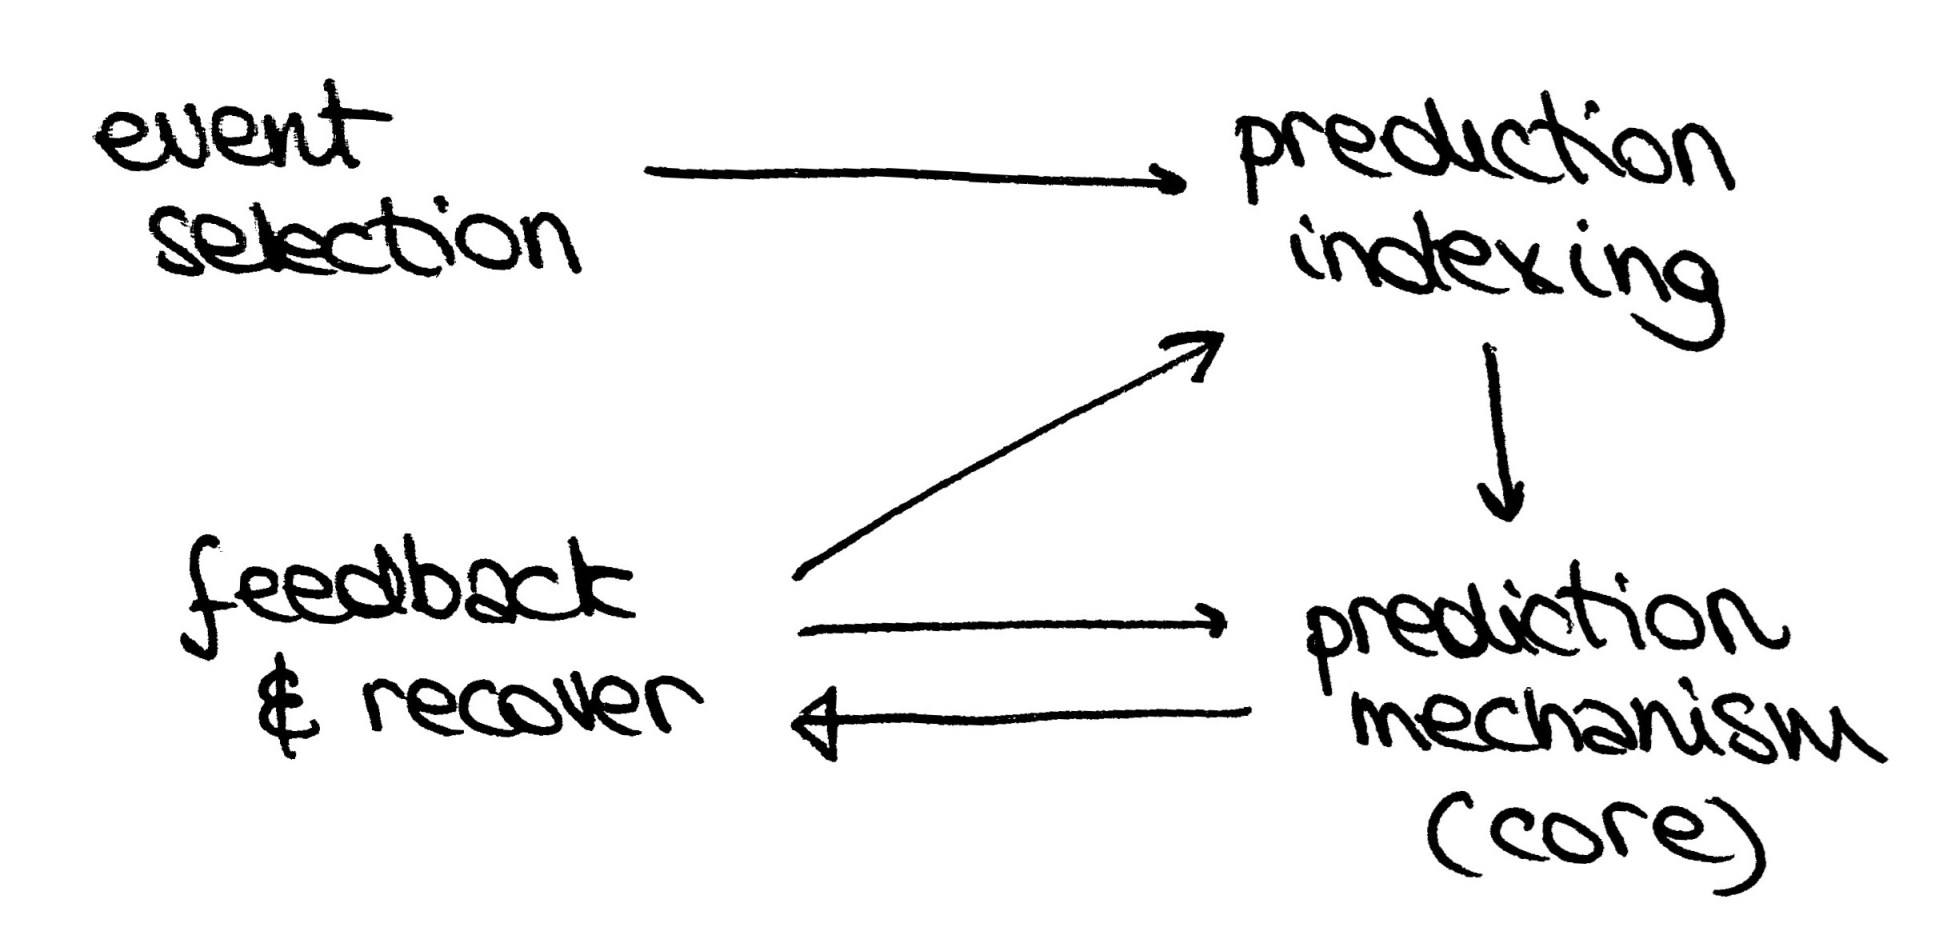
\includegraphics[width=0.55\linewidth]{img/img3/12}
\end{center}
This unit has to become active when one of the following events occur: branch,
call, jump or everything expecting the program counter not incrementing
sequentially.
Once we have run the prediction mechanism we have take a decision and after
some cycles we will know if the decision taken was correct or not, according to
this information the prediction algorithm can be made adaptive by updating
something in the prediction table. Different solutions can be exploited.
Depending on the algorithm, prediction technique can be static or dynamic.
%%%%%%%%%%%%%%%%%%%%%%%%%%%%%%%%%%%%%%%%%%%%%%%%%%%%%%%%%%%%%%%%%%%%%%%%%%%%%%%%
%%%%%%%%%%%%%%%%%%%%%%%%%%%%%%%%%%%%%%%%%%%%%%%%%%%%%%%%%%%%%%%%%%%%%%%%%%%%%%%%
%%%%%%%%%%%%%%%%%%%%%%%%%%%%%%%%%%%%%%%%%%%%%%%%%%%%%%%%%%%%%%%%%%%%%%%%%%%%%%%%
\subsection{Static prediction}
For every single branch a fixed direction is always predicted, the choice
regarding the direction is taken at compiler time or during profiling meaning
that if a certain branch is taken 80 \% of times than that branch will takes
always that direction. This solution is efficient in loops, for, while, etc
where almost of the time we remain inside the loop (in a 100-cycle for we are
correct for 100 times and the last we are wrong), for other kind of branches
this algorithm is correct for 66.6 \% of times, which is not actually so bad.
%%%%%%%%%%%%%%%%%%%%%%%%%%%%%%%%%%%%%%%%%%%%%%%%%%%%%%%%%%%%%%%%%%%%%%%%%%%%%%%%
%%%%%%%%%%%%%%%%%%%%%%%%%%%%%%%%%%%%%%%%%%%%%%%%%%%%%%%%%%%%%%%%%%%%%%%%%%%%%%%%
%%%%%%%%%%%%%%%%%%%%%%%%%%%%%%%%%%%%%%%%%%%%%%%%%%%%%%%%%%%%%%%%%%%%%%%%%%%%%%%%
\subsection{Dynamic prediction - 1 bit}
This solution is close to 80\% of right prediction.
Using the PC as address, we point to a certain location in the table and the
pointed value tells us if we have or not to take the branch. The value stored in
the cell is just the previous uotcome of the branch (0 untaken, 1 taken).
Nevertheless for many values of the PC (i.e. when instructions are not
branches) a lot of space is wasted in this memory. One possible idea is to not
use all $n$ bits of PC but just a subset made up of $k$ bits (excluding the two
LSB since they are related to the way we are addressing memory). In this way
some aliasing is present since we point to the same location in the table for
more than one instructions: by choosing $k$ small a lot of aliasing is present
instead by choosing it large less alias is present but the cost for the table
increases. A typical choice for $k$ is between 1000 and 4000.
\begin{center}
  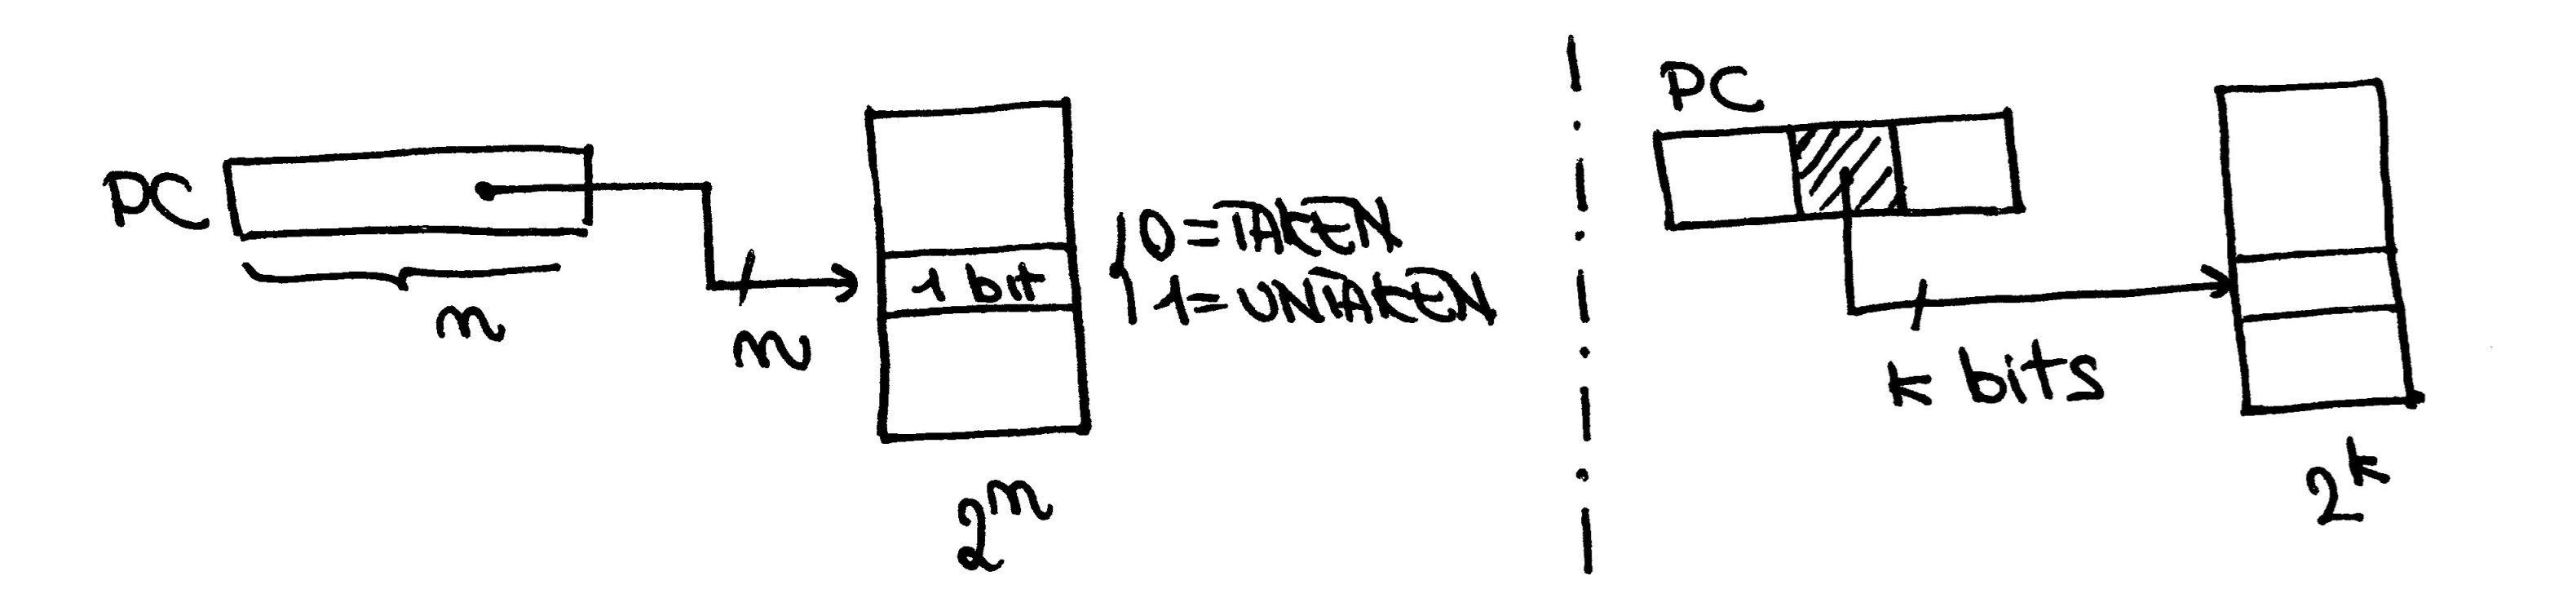
\includegraphics[width=0.75\linewidth]{img/img3/15}
\end{center}
Another alternative (in Intel architecture) is to adopt a cache-like
organization
\begin{center}
  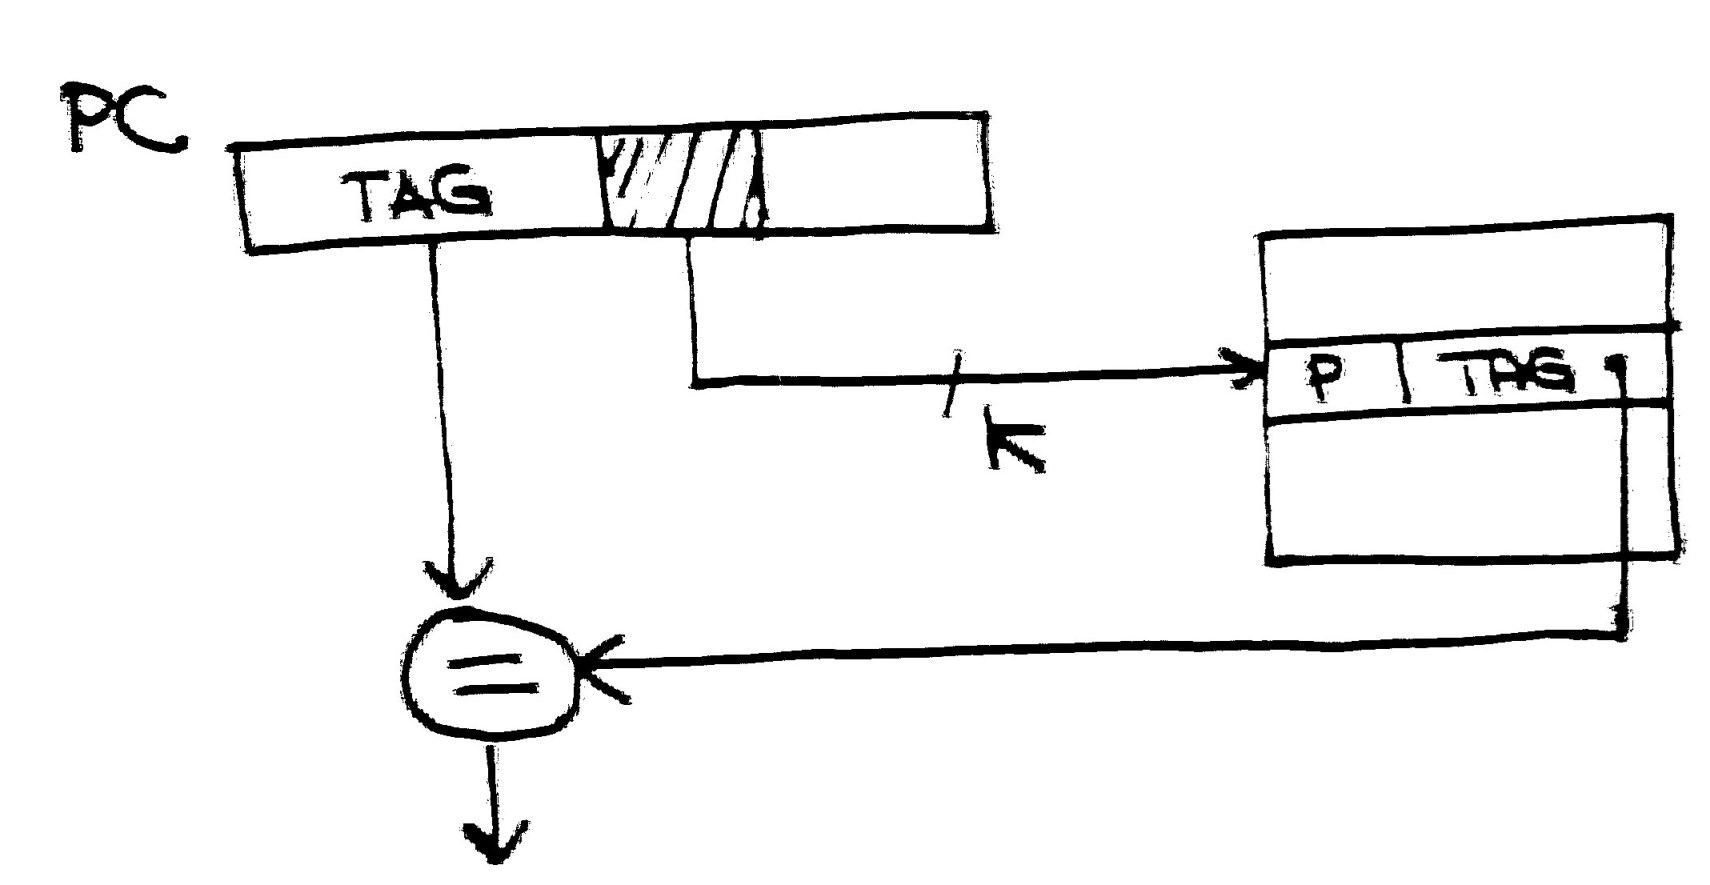
\includegraphics[width=0.6\linewidth]{img/img3/16}
\end{center}
The table is larger than the previous case and it is divided into two field:
left one is the same as before, right one corresponds to a tag. By comparing
table cell tag with the one in PC aliasing is avoided.\\
Independently on that, if we want to increase prediction mechanism performance
instead of using a single bit we can use 2 bits.
%%%%%%%%%%%%%%%%%%%%%%%%%%%%%%%%%%%%%%%%%%%%%%%%%%%%%%%%%%%%%%%%%%%%%%%%%%%%%%%%
%%%%%%%%%%%%%%%%%%%%%%%%%%%%%%%%%%%%%%%%%%%%%%%%%%%%%%%%%%%%%%%%%%%%%%%%%%%%%%%%
%%%%%%%%%%%%%%%%%%%%%%%%%%%%%%%%%%%%%%%%%%%%%%%%%%%%%%%%%%%%%%%%%%%%%%%%%%%%%%%%
\subsection{Dynamic prediction - 2 bit}
These 2 bits are used in order to represent 4 different scenarios:
\begin{enumerate}
  \item \textbf{ST} 11 \textit{strong taken}, so there is a high reliability
    on that.
  \item \textbf{WT} 10 \textit{weak taken}: the reliability for this choice
    is less than the previous one
  \item \textbf{SU} 01 \textit{strong untake}.
  \item \textbf{WU} 00 \textit{weak untake}.
\end{enumerate}
At the end of branch operation the prediction correctness has to be verified, a
certain amount of different cases may occurs. Depending on that the content of
memory is updated so that at the next occurrence of that particular instruction
we have a value for the prediction more right. The basic idea for updating the
memory content is:
\begin{itemize}
  \item Cell table content was ST and the branch was actually taken: in the
    table the value ST for that cell is confirmed.
  \item Cell table content was ST and the branch was actually not taken: in
    the table the new value for that cell is WT.
\end{itemize}
\begin{center}
  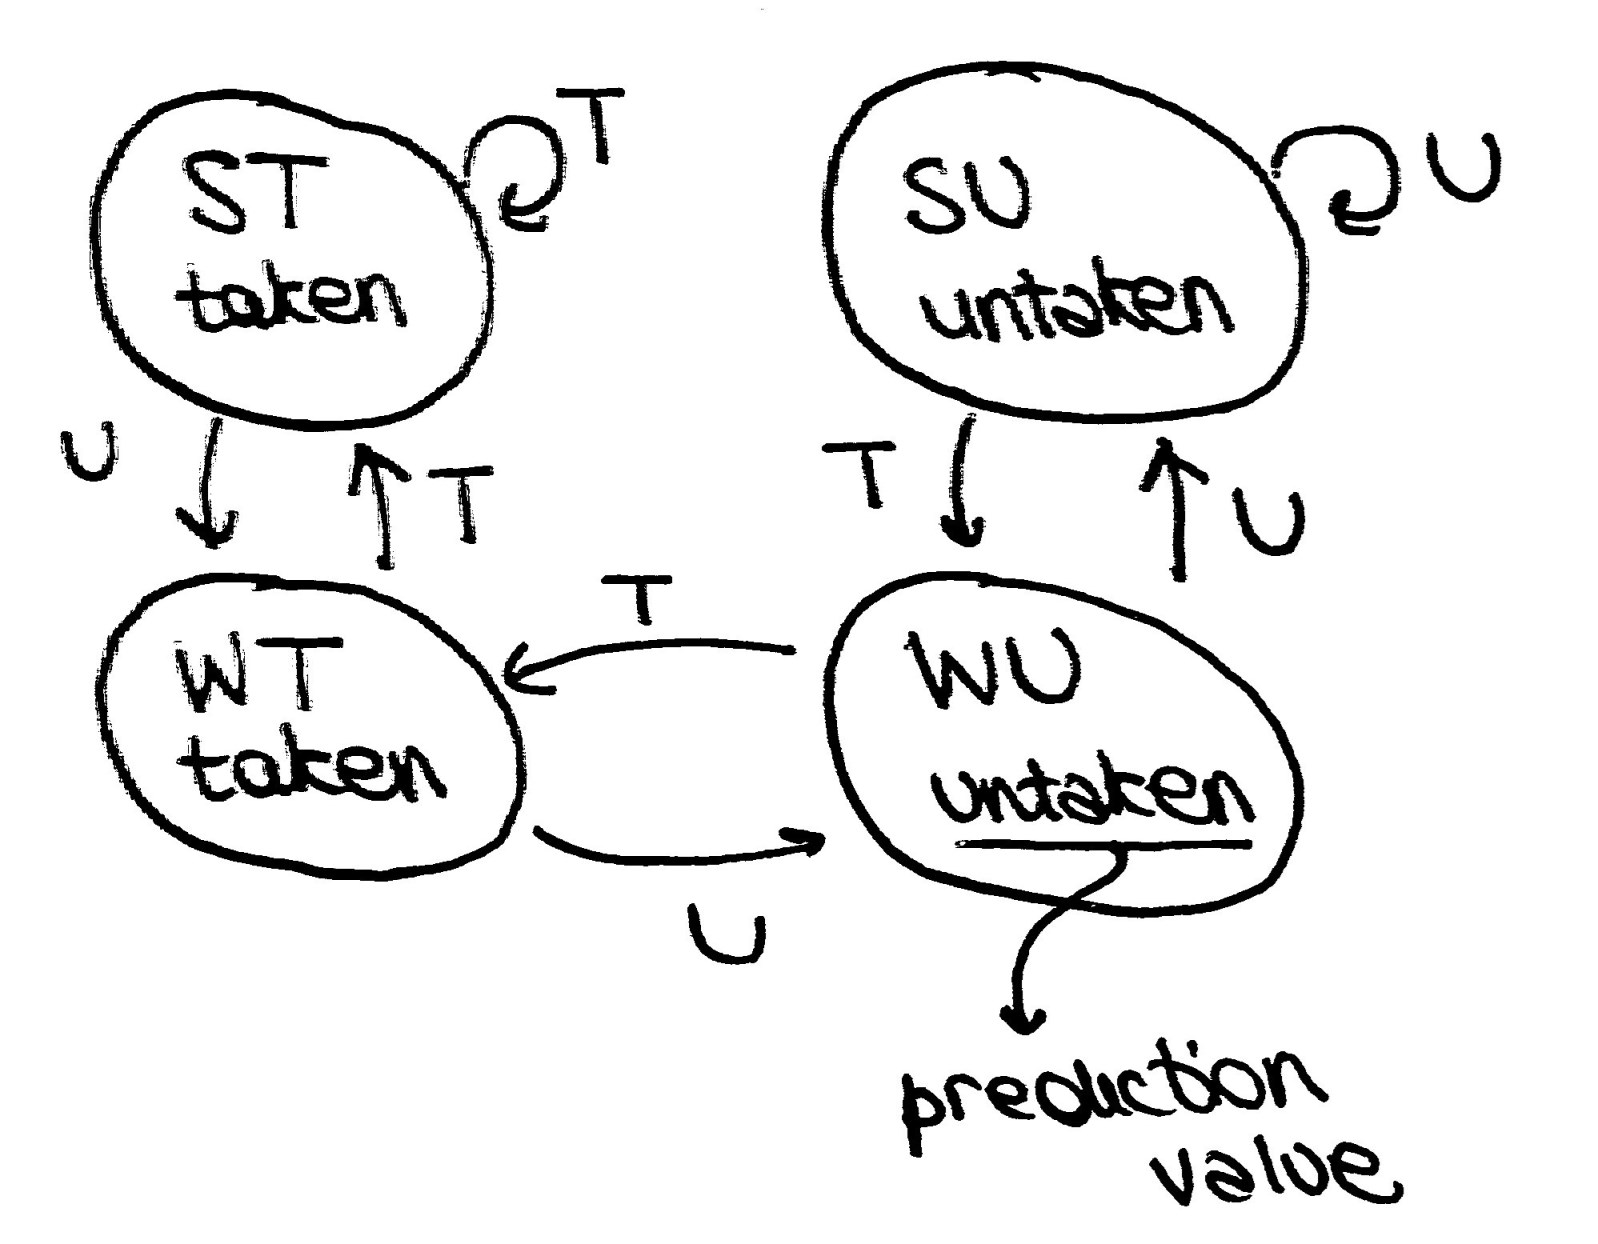
\includegraphics[width=0.6\linewidth]{img/img3/17}
\end{center}
\subparagraph{Example - nested loop}
Let's take the following piece of C-code:
\begin{verbatim}
for (i=0; i < n; i++)
    for(j=0; j<m, j++)
        ...
\end{verbatim}
\textbf{One bit prediction}: at the end of inner loop (i, j=m-1) we predict
taken but it was actually un-taken, so at the next operation we predict un-taken
but actually we have to take the branch (i+1, j=0).\\
\textbf{2-bit prediction}: at the last iteration of inner loop we predict taken
but it was untake, so actually that instruction will be associated to weak taken
and at the following occurrence (i+1, j=0) the prediction will be correct. 2-bit
prediction has a limited extra cost with respect to one bit but in nested loop
it has a -50 \% of wrong prediction (1 case instead of 2).\\
Using 2-bit prediction we are clore to 90\% right prediction.
\subparagraph{Example - correlated branches}
Another way to improve predictor performance is in the case of correlated
branches, so when one branch depends on the direction of one or multiple
previous branches.
\begin{verbatim}
if (a==2)
    aa=0;
if(b=2);
    bb=0;
if (aa !=bb) {
  ...
}
\end{verbatim}
In this case three branches are present, in the last one direction depends on
previous taken directions, meaning that if both branch 1 and 2 have been taken
then branch 3 will not.
They are not statically independent each other, we should be able to detect this
kind of situation to be able to significantly improve our performance So far the
table was indexed by PC, so it is a local prediction (just considering a single
branch instruction), using this approach it is not possible consider more than
one branch at the same time, this implies that a different structure has to be
employed.
%%%%%%%%%%%%%%%%%%%%%%%%%%%%%%%%%%%%%%%%%%%%%%%%%%%%%%%%%%%%%%%%%%%%%%%%%%%%%%%%
%%%%%%%%%%%%%%%%%%%%%%%%%%%%%%%%%%%%%%%%%%%%%%%%%%%%%%%%%%%%%%%%%%%%%%%%%%%%%%%%
%%%%%%%%%%%%%%%%%%%%%%%%%%%%%%%%%%%%%%%%%%%%%%%%%%%%%%%%%%%%%%%%%%%%%%%%%%%%%%%%
\subsection{Global scheme}
Moving to a new scheme, called "global", key point is to have a kind of shift
register where every new instruction to be predicted is inserted at the right
and then content is shifted, in particular for a certain instruction we insert
0 or 1 depending if in the last occurrence that branch was taken or not. Finally
this register is employed to indexed the prediction table, now called Pattern
History Table.\\
The key different with respect to local scheme is that in order to index the
prediction table we use outcomes of previous branches operations, so it is like
using a snapshot of last operations.
\begin{center}
  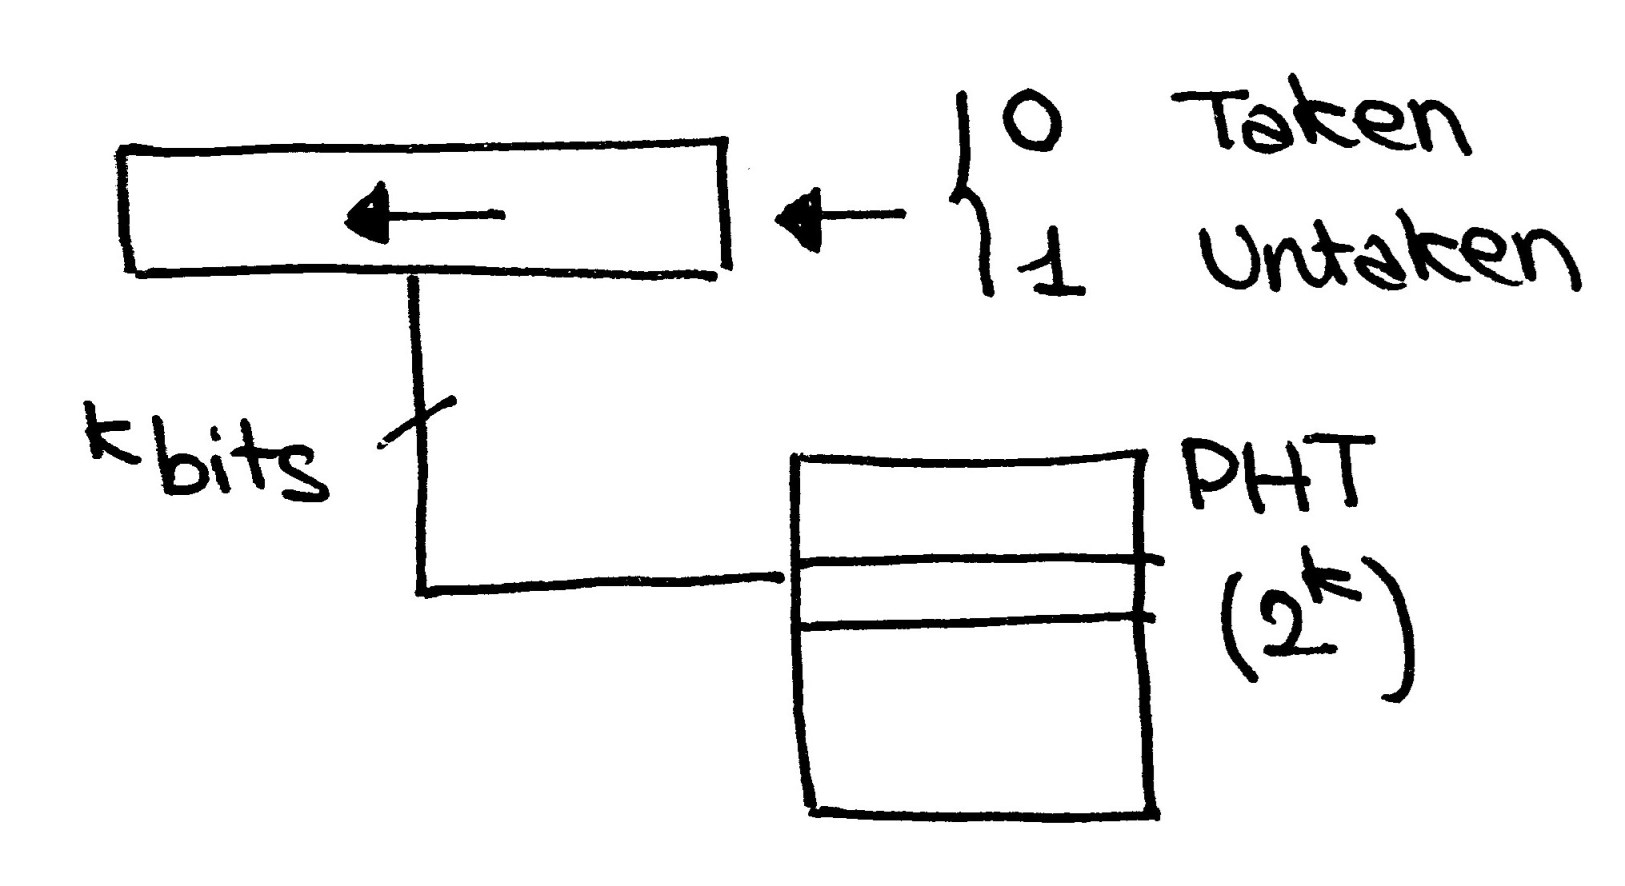
\includegraphics[width=0.6\linewidth]{img/img3/19}
\end{center}
\large{NOTE: 0 is untaken, 1 is taken}
% Coming back to the last example, we notice that:
% \begin{center}
%   \begin{tabular}{|c|c|c|}
%     \hline
%     Branch 1&   Branch 2&   Branch 3\\
%     \hline
%     taken&      taken&      untaken\\
%     0&          0&      1\\
%     \hline
%   \end{tabular}
% \end{center}
% So with a double 0 the third digit has to be 1. if k=2, ... todo mancante...
% This implementation is very efficient when there is some correlation, but when 
% there is no correlation the location prediction is much better, so a good idea 
% is to mix them together.
%%%%%%%%%%%%%%%%%%%%%%%%%%%%%%%%%%%%%%%%%%%%%%%%%%%%%%%%%%%%%%%%%%%%%%%%%%%%%%%%
%%%%%%%%%%%%%%%%%%%%%%%%%%%%%%%%%%%%%%%%%%%%%%%%%%%%%%%%%%%%%%%%%%%%%%%%%%%%%%%%
%%%%%%%%%%%%%%%%%%%%%%%%%%%%%%%%%%%%%%%%%%%%%%%%%%%%%%%%%%%%%%%%%%%%%%%%%%%%%%%%
\subsection{G-share (Local + Global scheme)}
\subparagraph{Global-global}
\begin{center}
  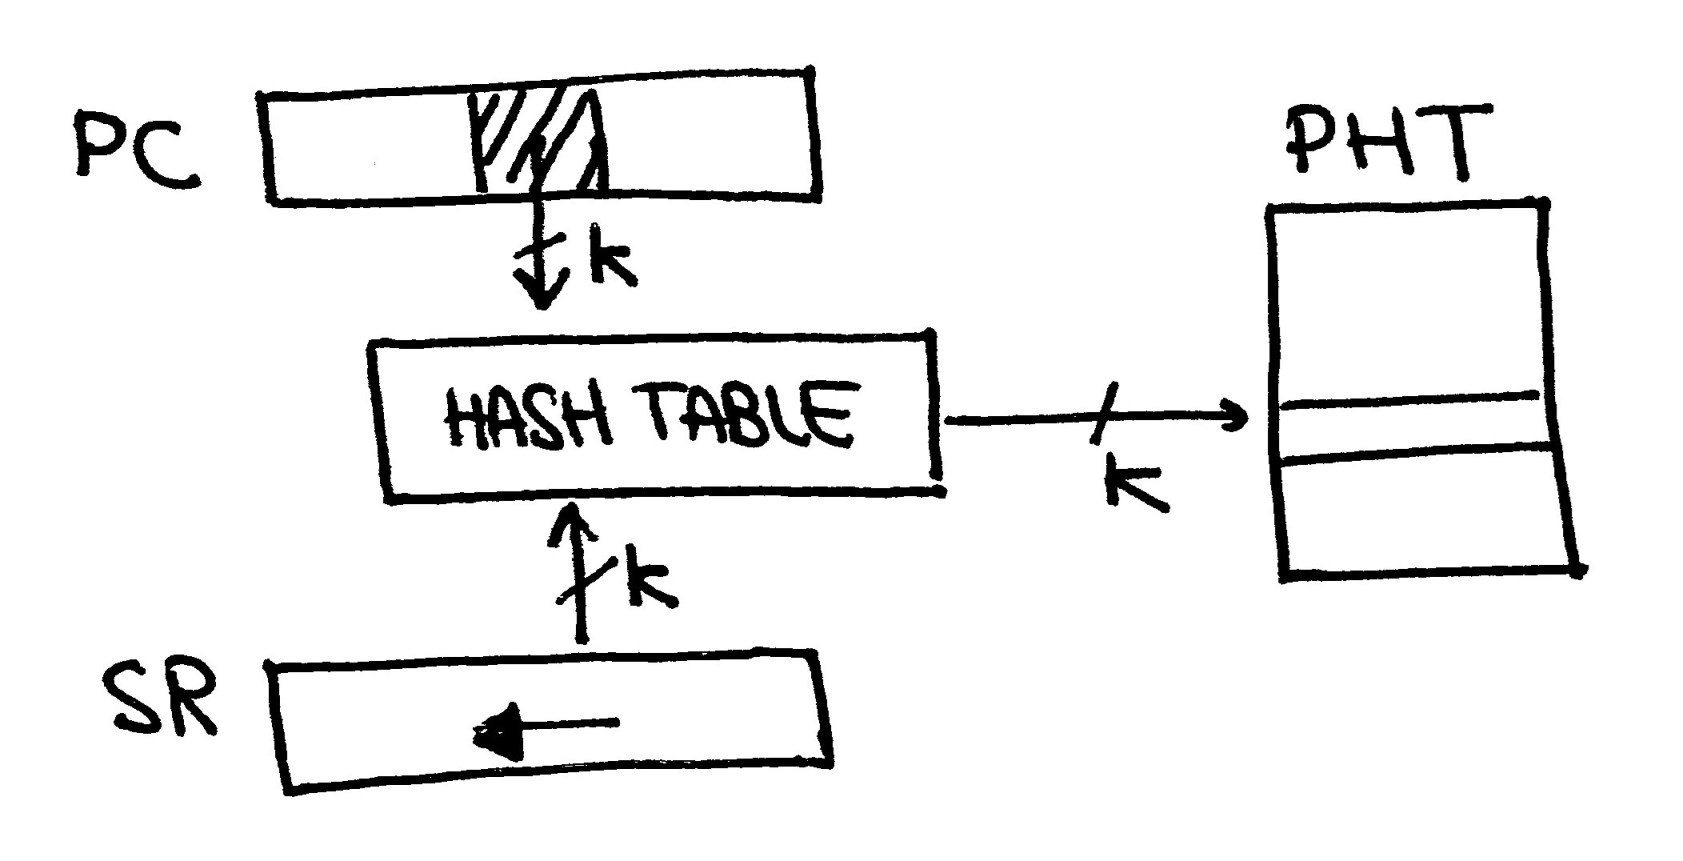
\includegraphics[width=0.6\linewidth]{img/img3/20}
\end{center}
We mix together PC (local address) and shift register (global information)
using an hash table which output is employed to point at PHT(pattern history
table). One very simple implementation for hash is performing a xor bit a bit
between two inputs data.  In order to reduce aliasing we can increase $k$ or
get more complex schemes.
\newpage
\subparagraph{Global-set}
\begin{center}
  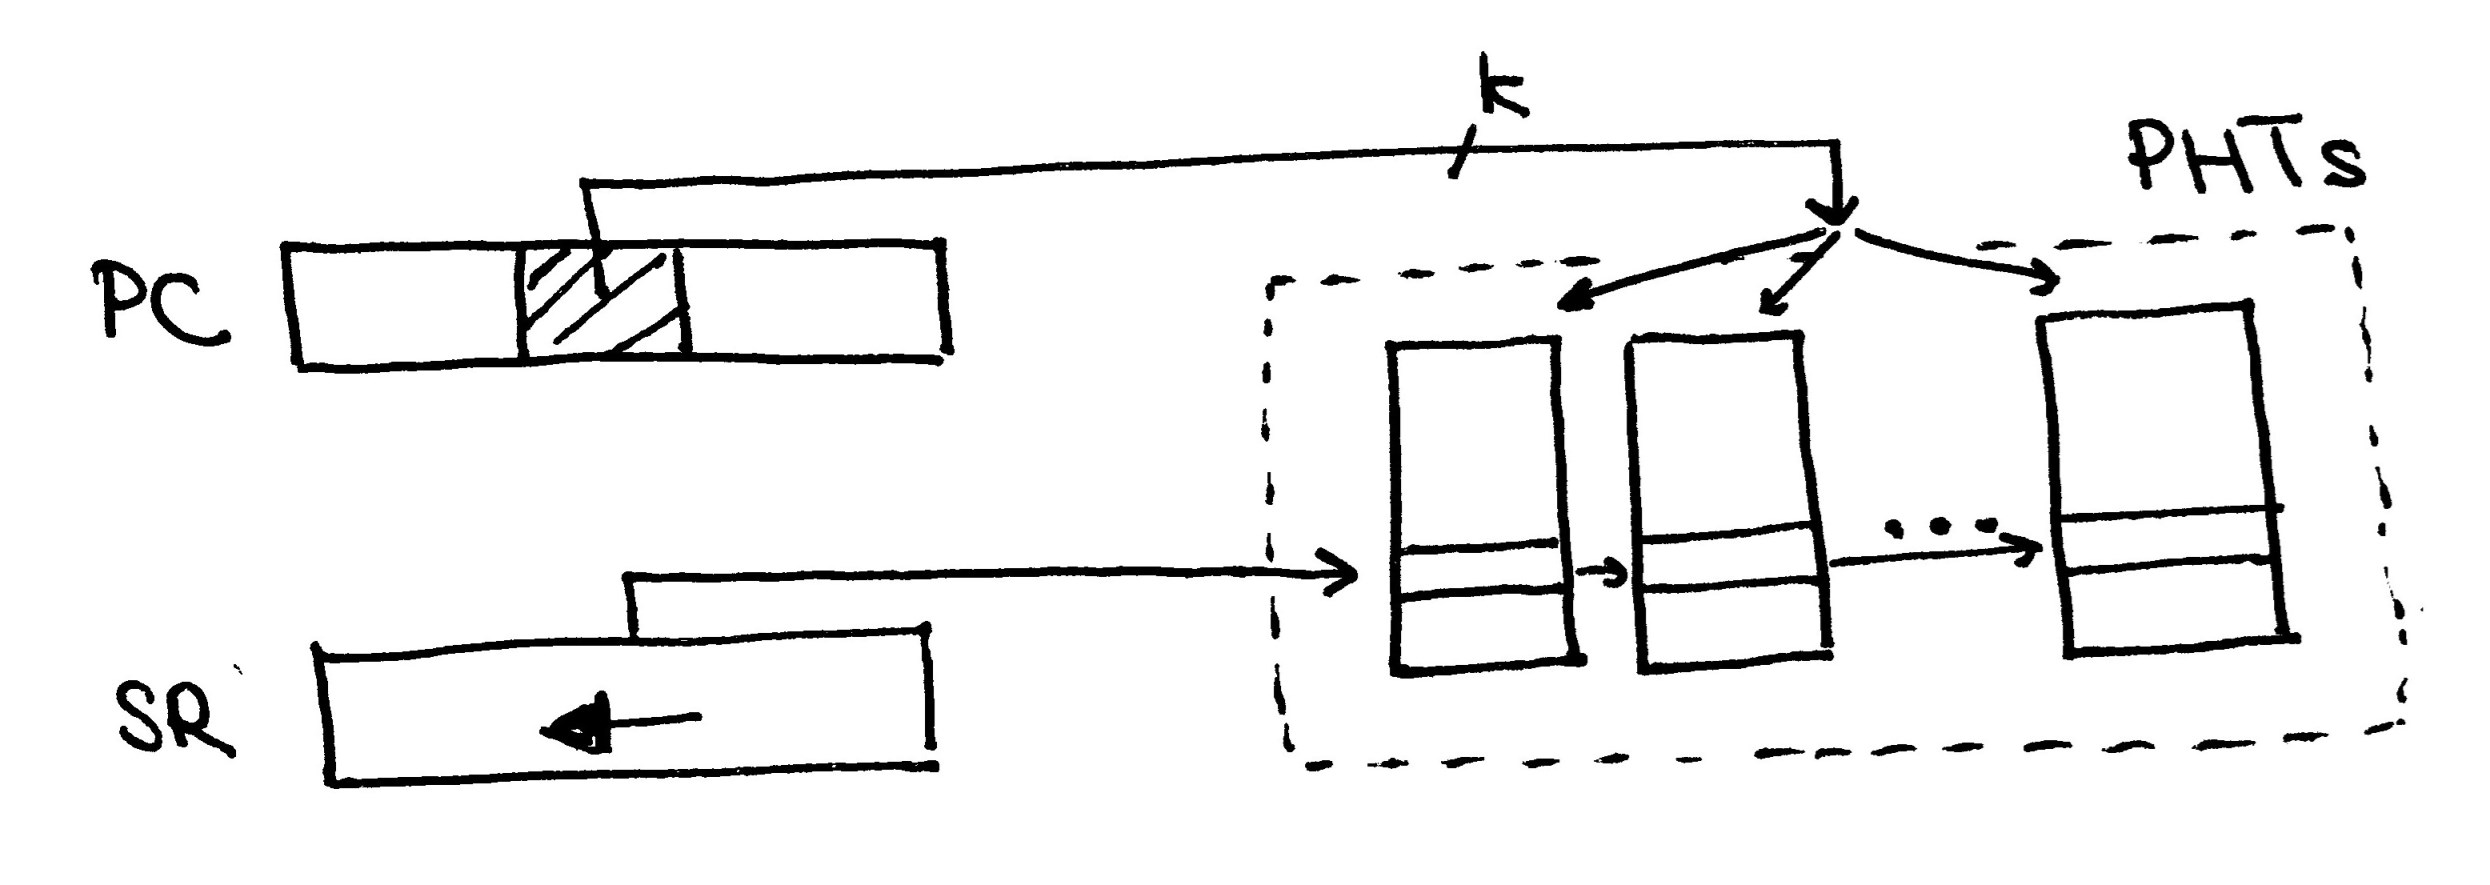
\includegraphics[width=0.7\linewidth]{img/img3/21}
\end{center}
There are separate tables for each branch instruction, so by using $k$ bits
from PC we select the corresponding PHT and then we use the Shift Register to
make an access to the selected PHT. Aliasing is resolved but cost has
noticeably increase.
\subparagraph{Set-global}
\begin{center}
  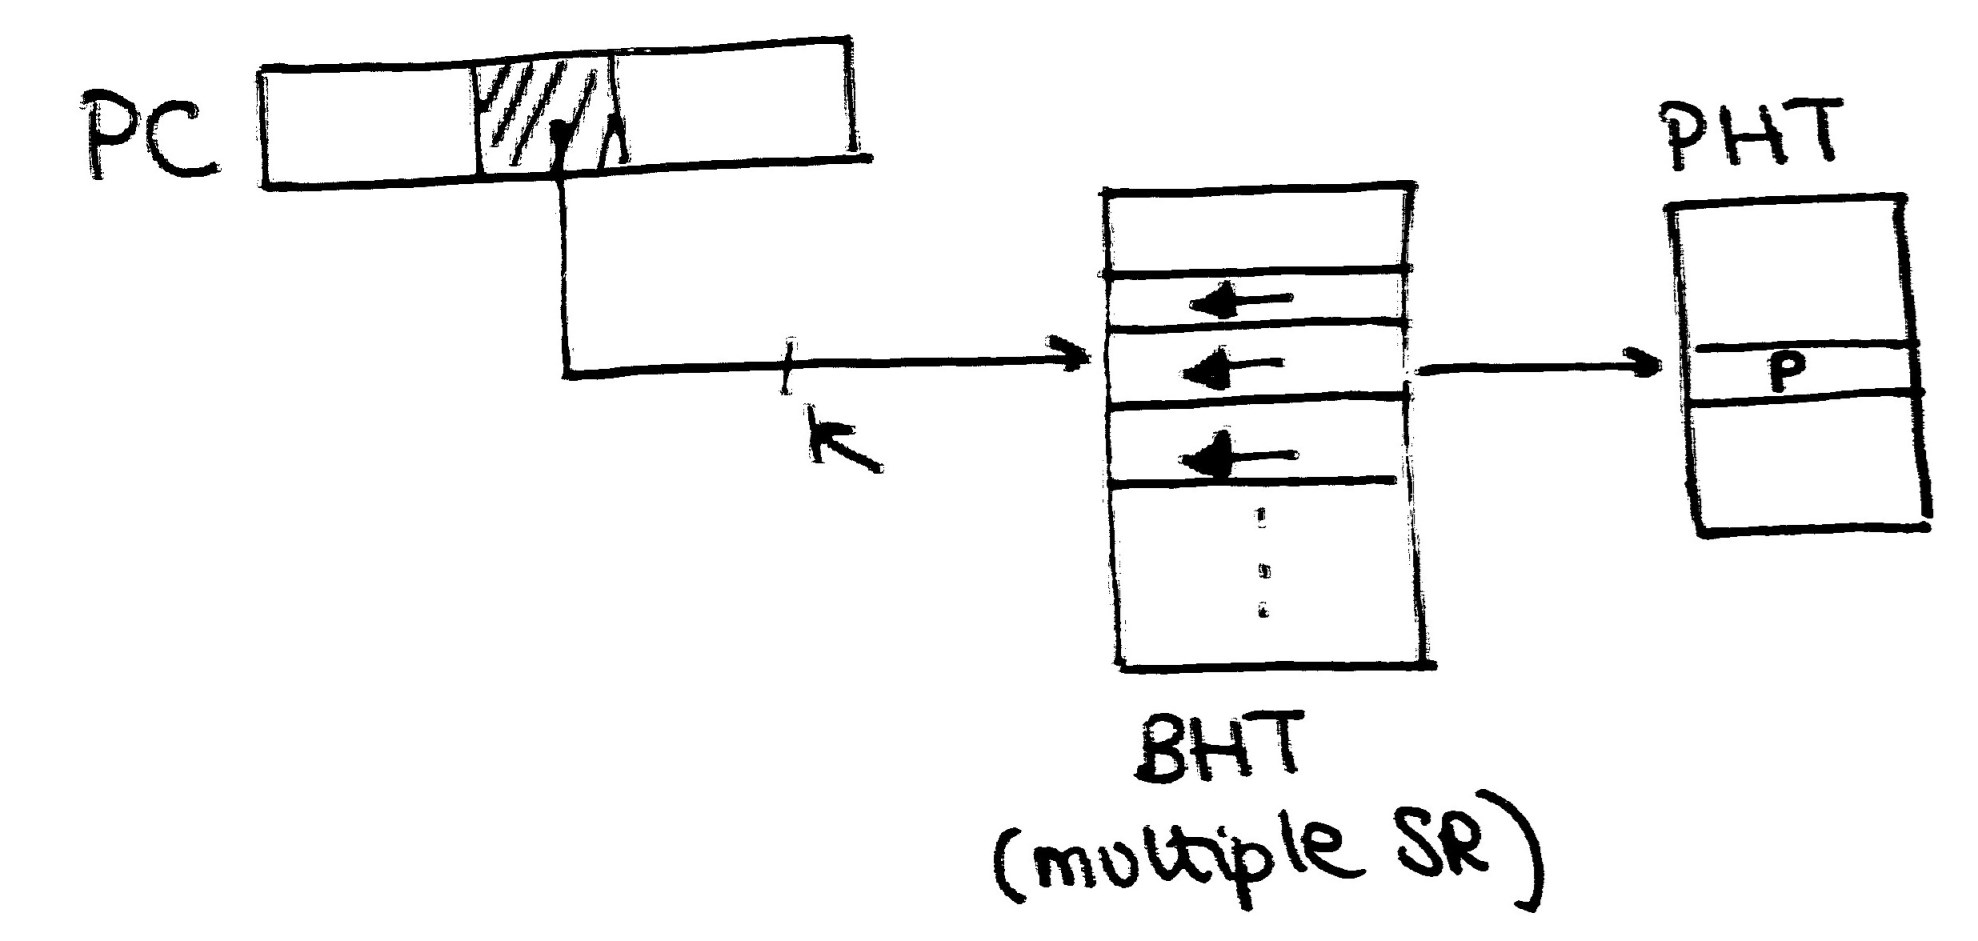
\includegraphics[width=0.7\linewidth]{img/img3/22}
\end{center}
One single PHT but many SR.
\subparagraph{Set-set}
\begin{center}
  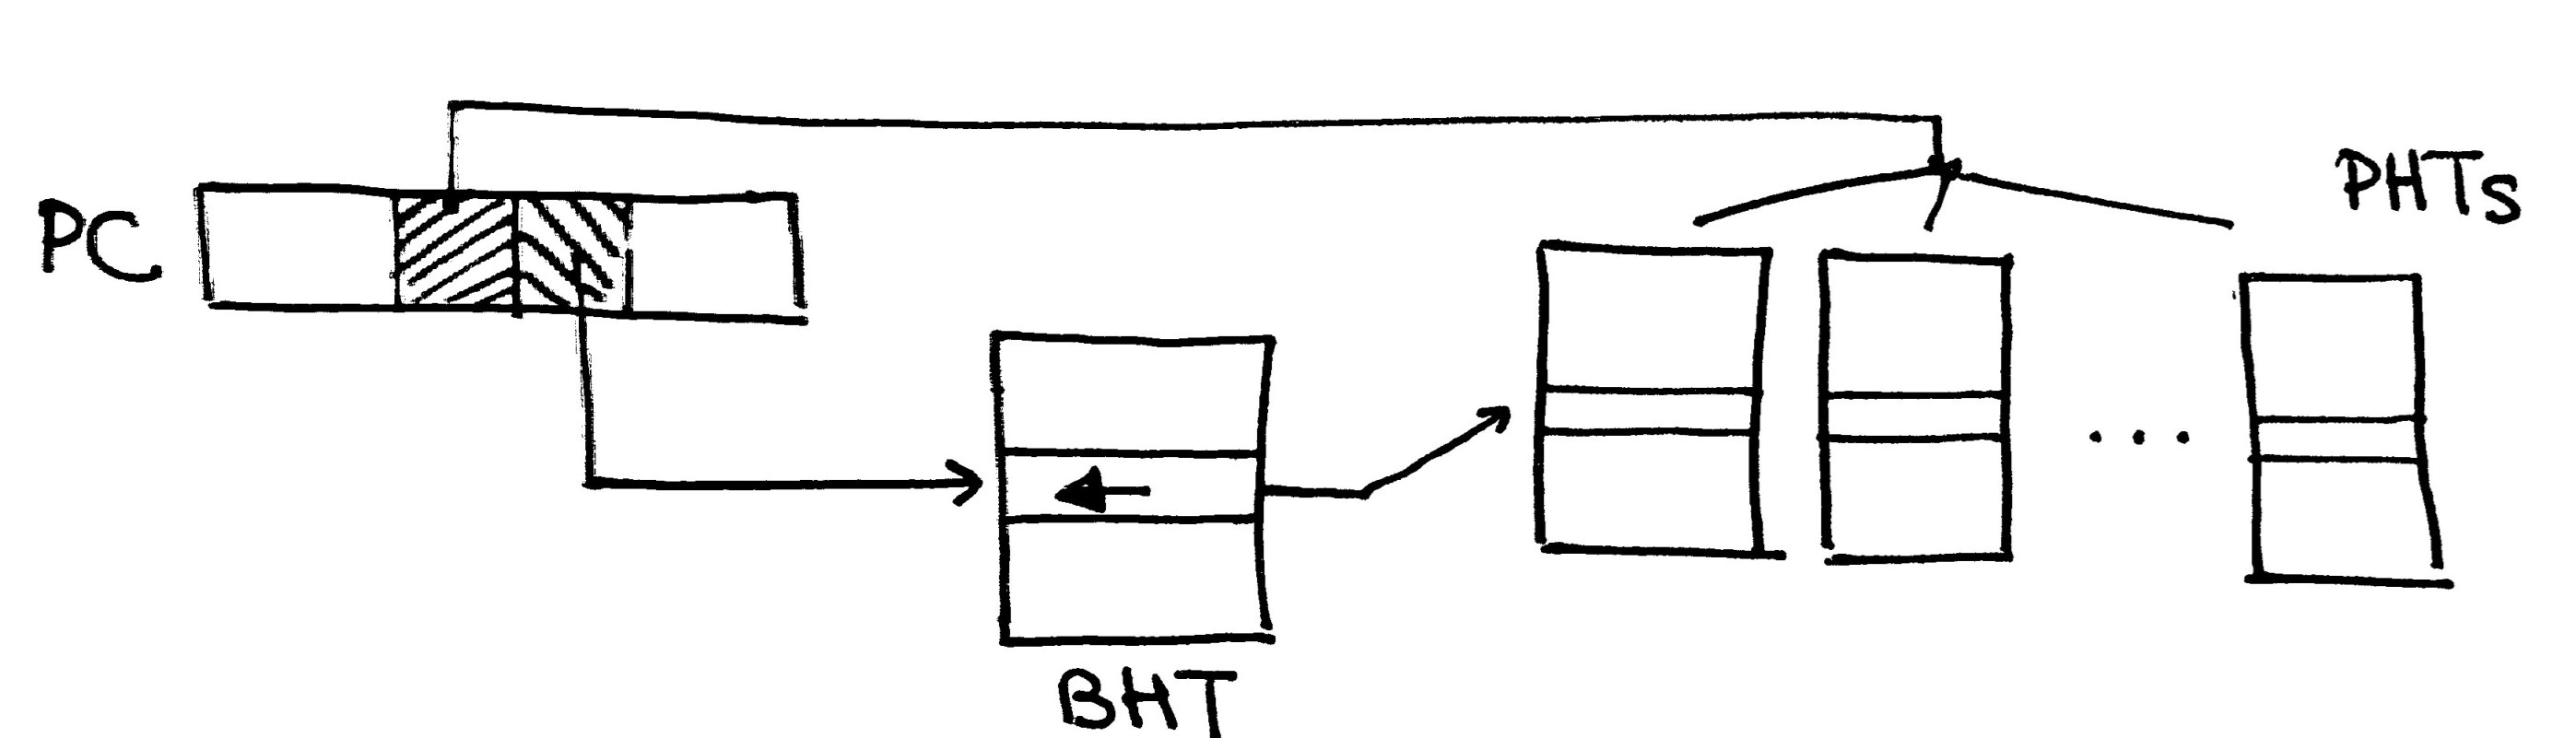
\includegraphics[width=0.7\linewidth]{img/img3/23}
\end{center}
Bits coming from PC are separated into two fields, this solution reduces
aliasing more than the other schemes but it also the more expensive.
%%%%%%%%%%%%%%%%%%%%%%%%%%%%%%%%%%%%%%%%%%%%%%%%%%%%%%%%%%%%%%%%%%%%%%%%%%%%%%%%
%%%%%%%%%%%%%%%%%%%%%%%%%%%%%%%%%%%%%%%%%%%%%%%%%%%%%%%%%%%%%%%%%%%%%%%%%%%%%%%%
%%%%%%%%%%%%%%%%%%%%%%%%%%%%%%%%%%%%%%%%%%%%%%%%%%%%%%%%%%%%%%%%%%%%%%%%%%%%%%%%
\newpage
\subsection{Hybrid prediction}
Let's imagine to have more than one predictors and a meta-predictor choosing
dynamically which predictor which one has to be used.
\begin{center}
  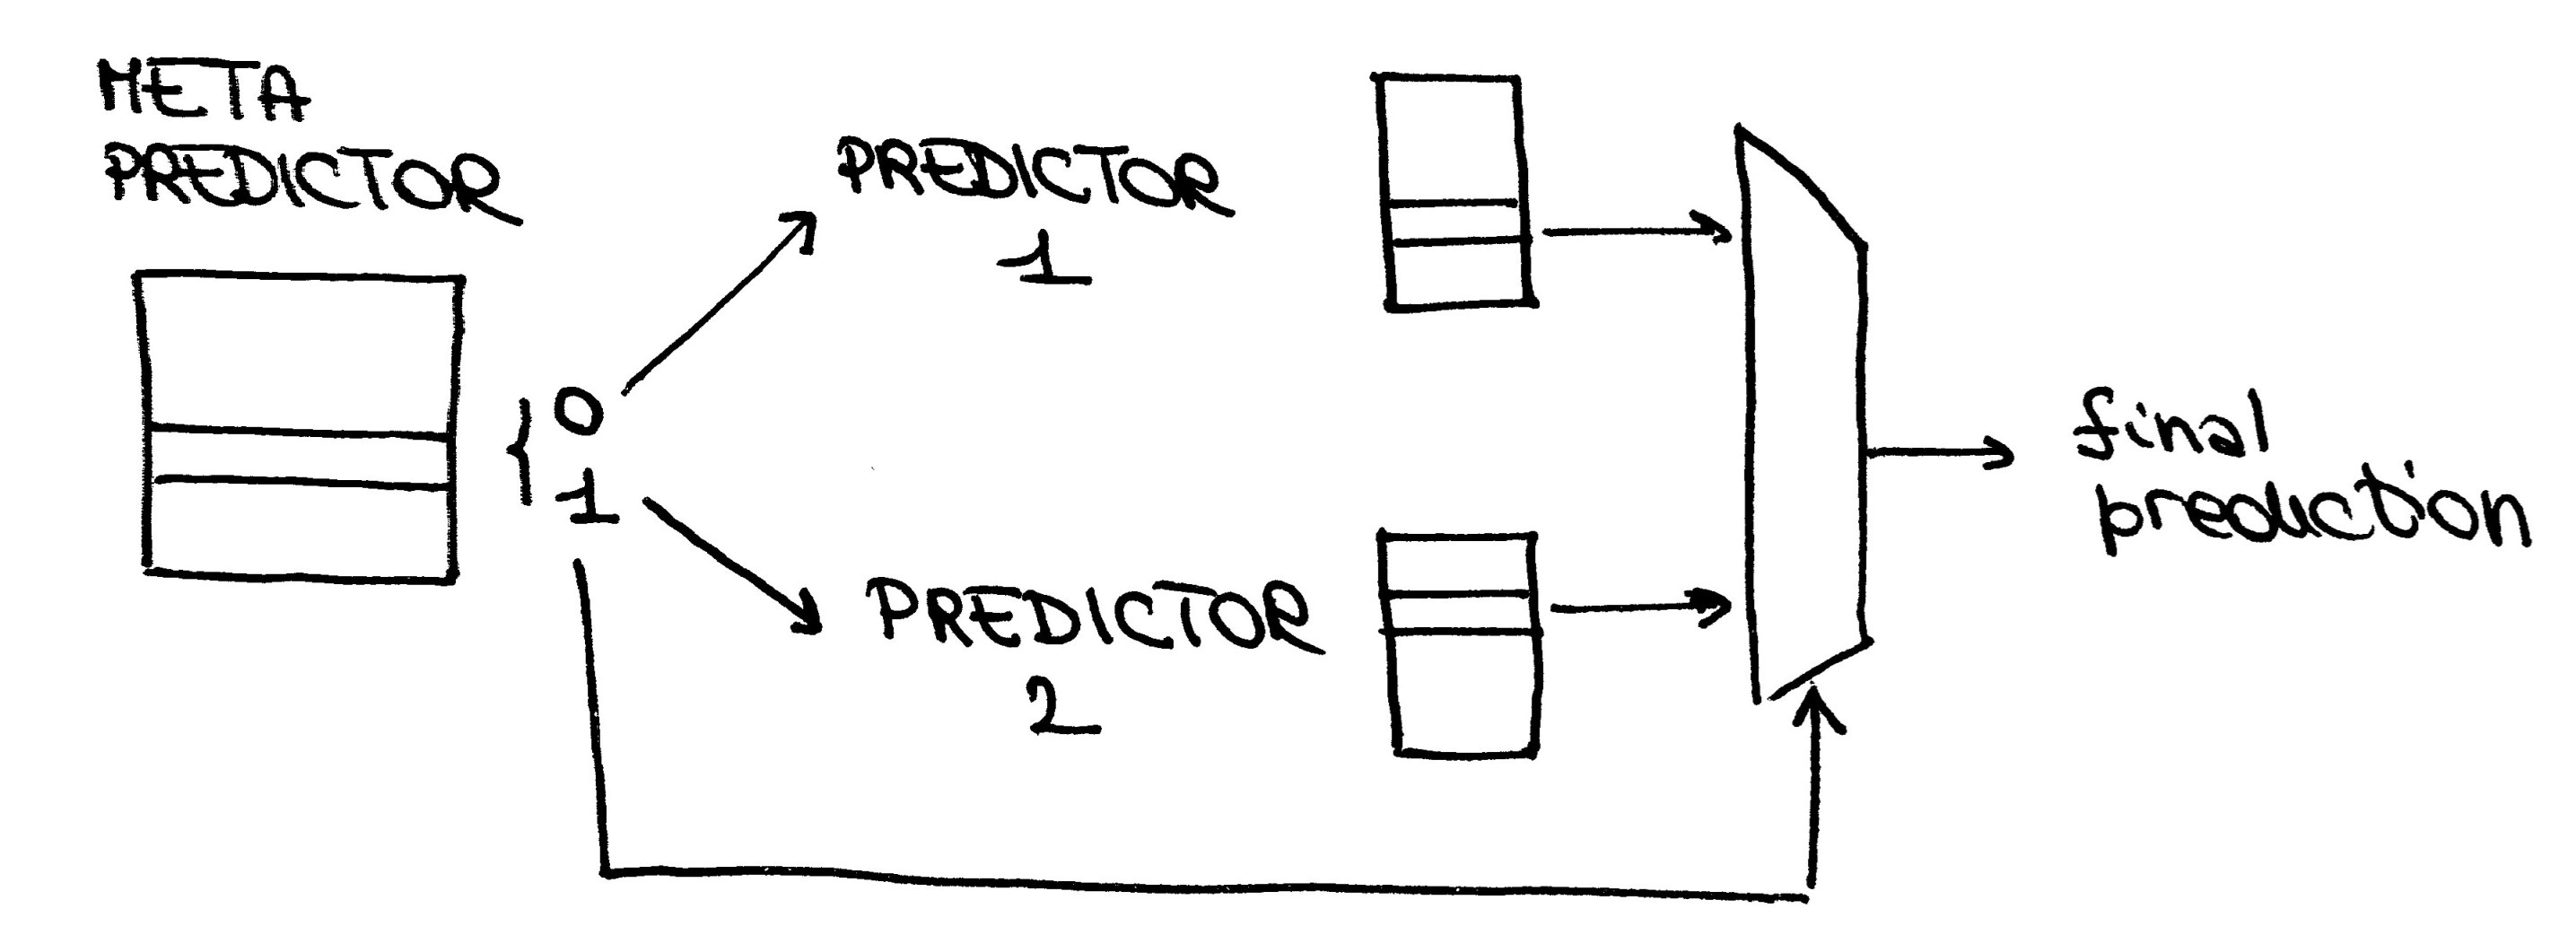
\includegraphics[width=0.7\linewidth]{img/img3/24}
\end{center}
Starting from two predictors, maybe predictor 1 is better in some cases while
predictor 2 is better for other: meta-predictor has to choose the proper one.
For example if predictor 2 is a global one and the current branch is correlated
to other predictions/branches, probably the best choice consists of using this
one.
%%%%%%%%%%%%%%%%%%%%%%%%%%%%%%%%%%%%%%%%%%%%%%%%%%%%%%%%%%%%%%%%%%%%%%%%%%%%%%%%
%%%%%%%%%%%%%%%%%%%%%%%%%%%%%%%%%%%%%%%%%%%%%%%%%%%%%%%%%%%%%%%%%%%%%%%%%%%%%%%%
%%%%%%%%%%%%%%%%%%%%%%%%%%%%%%%%%%%%%%%%%%%%%%%%%%%%%%%%%%%%%%%%%%%%%%%%%%%%%%%%
\subsection{Target address prediction}
It is not sufficient to determine the direction of branch, we also need to
predict the target address since it takes time for the processor to compute
it (we want only at the end verify if the direction of the branch and the
target address are fine, so that in the meanwhile we are doing hopefully useful
things).
A simple idea is to point to a table having two fields:
\begin{itemize}
  \item Branch direction (1 or 2 bits).
  \item Target address.
\end{itemize}
At the beginning everything is empty so it's really a guess for the direction,
once the instruction has been completed we save the actual value for the
direction and the target address so that at the next occurrence of that
instruction we have everything already ready.
\begin{center}
  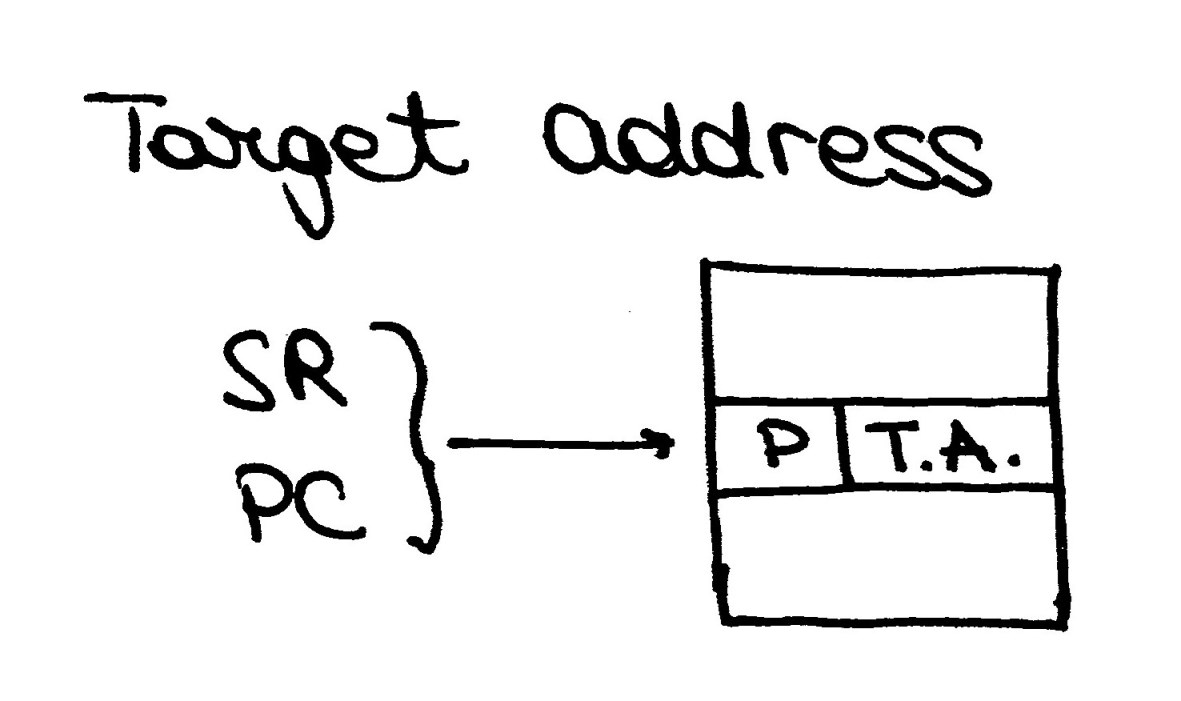
\includegraphics[width=0.5\linewidth]{img/img3/25}
\end{center}
